% -*-latex-*-

\chapter{Analysis}
\label{C7}

For E08-027, asymmetries and unpolarized cross-sections are measured to extract the polarized cross-section differences for polarized inclusive electron scattering. These quantities are measured with a polarized electron beam and a polarized NH${}_3$ target as we already discussed in \Cref{C5}. This chapter will give an overview of the analysis of the necessary inputs to extract the polarized cross-section differences.

\section{Asymmetries and Cross-Sections}
\label{C7S1}

The physics asymmetries are calculated by taking the ratio of the polarized cross-section difference to the polarized cross-section sum. The longitudinal and transverse asymmetries can be expressed as:
\begin{equation} \label{C7S1E1}
A_{\parallel}=\cfrac{\frac{\dd[2]{\sigma}^{\buildrel\leftarrow\over\Rightarrow}}{\dd{\Omega}\dd{E'}}-\frac{\dd[2]{\sigma}^{\buildrel\rightarrow\over\Rightarrow}}{\dd{\Omega}\dd{E'}}}{\frac{\dd[2]{\sigma}^{\buildrel\leftarrow\over\Rightarrow}}{\dd{\Omega}\dd{E'}}+\frac{\dd[2]{\sigma}^{\buildrel\rightarrow\over\Rightarrow}}{\dd{\Omega}\dd{E'}}},
\end{equation}
and
\begin{equation} \label{C7S1E2}
A_{\perp}=\cfrac{\frac{\dd[2]{\sigma}^{\leftarrow\Uparrow}}{\dd{\Omega}\dd{E'}}-\frac{\dd[2]{\sigma}^{\rightarrow\Uparrow}}{\dd{\Omega}\dd{E'}}}{\frac{\dd[2]{\sigma}^{\leftarrow\Uparrow}}{\dd{\Omega}\dd{E'}}+\frac{\dd[2]{\sigma}^{\rightarrow\Uparrow}}{\dd{\Omega}\dd{E'}}},
\end{equation}
where $\leftarrow$ and $\rightarrow$ refer to the electron spin pointing either parallel or anti-parallel to the momentum direction, $\Rightarrow$ indicates that the target is longitudinally polarized and $\Uparrow$ designates that the target is transversely polarized.

The raw asymmetries are calculated using the number of events within the $\pm$ helicity state:
\begin{equation} \label{C7S1E3}
A_{\mathrm{raw}}=\frac{\frac{N^+}{LT^+Q^+}-\frac{N^-}{LT^-Q^-}}{\frac{N^+}{LT^+Q^+}+\frac{N^-}{LT^-Q^-}},
\end{equation}
where $N^\pm$ is the number of events, $LT^{\pm}$ is the livetime and $Q^\pm$ is the charge in the $\pm$ helicity state respectively.

The physics asymmetries and the raw asymmetries are related through the expression:
\begin{equation} \label{C7S1E4}
A_{\parallel,\perp}^{\mathrm{phys}}=\frac{A_{\parallel,\perp}^{\mathrm{raw}}}{fP_bP_t},
\end{equation}
where $f$ is the dilution factor due to the unpolarized nitrogen and helium nuclei in the target, $P_b$ is the beam polarization and $P_t$ is the target polarization.

Due to the radiation effect, we need to make radiative corrections to \cref{C7S1E4} to retrieve Born asymmetries:
\begin{equation} \label{C7S1E5}
A_{\parallel,\perp}^{\mathrm{Born}}=A_{\parallel,\perp}^{\mathrm{phys}}+\Delta A_{\mathrm{RC}}^{\mathrm{ext}}+\Delta A_{\mathrm{RC}}^{\mathrm{int}},
\end{equation}
where $\Delta A_{\mathrm{RC}}^{\mathrm{ext}}$ and $\Delta A_{\mathrm{RC}}^{\mathrm{int}}$ are the external and internal radiative corrections respectively.

The raw unpolarized cross-section can be expressed in terms of measurable quantities as:
\begin{equation} \label{C7S1E6}
\sigma_0^{\mathrm{raw}} = \cfrac{\cfrac{ps\cdot N}{LT\cdot\eta_{\mathrm{det}}}}{\cfrac{Q}{e}\cdot\rho\cdot\Delta Z }\cdot\frac{1}{\Delta\Omega\Delta E'},
\end{equation}
where
\begin{itemize}[parsep=0pt]
\item $N$ is the number of detected electrons within the acceptance and the particle identification cuts;
\item $ps$ is the prescale factor for the DAQ system;
\item $LT$ is the livetime defined in \Cref{C5S4SS2};
\item $\eta_{\mathrm{det}}$ is the product of all hardware and software detector efficiencies;
\item $Q$ is the total charge read by BCMs, $e$ is the electron charge;
\item $\rho$ is the target density;
\item $\Delta Z$ is the target length seen by the spectrometer;
\item $\Delta\Omega$, $\Delta E'$ are the solid angle acceptance and the momentum acceptance.
\end{itemize}

The contribution from materials other than hydrogen in the target must be removed from the raw cross-section:
\begin{equation} \label{C7S1E7}
\sigma_0^{\mathrm{phys}} = \sigma_0^{\mathrm{raw}}\cdot f,
\end{equation}
where $f$ is the dilution factor. The unpolarized Born cross-section can be determined after applying the external and internal radiative corrections:
\begin{equation} \label{C7S1E8}
\sigma_0^{\mathrm{Born}} = \sigma_0^{\mathrm{phys}}+\Delta \sigma_{\mathrm{RC}}^{\mathrm{ext}}+\Delta \sigma_{\mathrm{RC}}^{\mathrm{int}}.
\end{equation}

The corss-section differences can be expressed as the product of the physics asymmetries and the unpolarized cross-sections:
\begin{equation} \label{C7S1E9}
\Delta\sigma_{\parallel,\perp}^{\mathrm{phys}} = 2A_{\parallel,\perp}^{\mathrm{phys}}\cdot\sigma_0^{\mathrm{phys}}.
\end{equation}

\section{Detector Efficiencies}
\label{C7S2}

The detector efficiency $\epsilon_{\mathrm{det}}$ in \cref{C7S1E6} contains several different contributions:
\begin{equation} \label{C7S2E1}
\eta_{\mathrm{det}} = \eta_{\mathrm{VDC}}\cdot\eta_{\mathrm{trigger}}\cdot\eta_{\mathrm{PID}},
\end{equation}
where $\eta_{\mathrm{VDC}}$ is the VDC efficiency, $\eta_{\mathrm{det}}$ is the trigger efficiency and the $\eta_{\mathrm{PID}}$ is the particle identification (PID) efficiency determined by the performance of the Cherenkov detector and the lead-glass calorimeters. The trigger efficiency has been discussed in \Cref{C5S4SS2}. In this section, we will discuss VDC efficiency and the PID efficiency.

\subsection{VDC Efficiency}
\label{C7S2SS1}

The efficiency of the VDCs is defined as:
\begin{equation} \label{C7S2E2}
\eta_{\mathrm{VDC}} = \frac{N_{\mathrm{good}}}{N_{\mathrm{total}}},
\end{equation}
where $N_{\mathrm{good}}$ is the number of the events with at least one track reconstructed by VDC and verified with calorimeters, and $N_{\mathrm{total}}$ is the number of total accepted events.

Under normal conditions, detected particle leaves only one track in the HRS detectors. However, multi-track events can occur when several particles pass through the wire chambers simultaneously or due to noise. Only events with a single track are kept in the cross-section analysis for convenience, thus the results need to be corrected for the efficiency due to the presence of multi-track events, which is defined as:
\begin{equation} \label{C7S2E3}
\eta_{\mathrm{multitrack}} = \frac{N_{\mathrm{onetrack}}}{N_{\mathrm{total}}},
\end{equation}
where $N_{\mathrm{onetrack}}$ is the number of the events with only one track reconstructed by VDC. The fraction of multi-track events was small when the event rate is low. However, the fraction of multi-track events reached 30\% in some kinematic settings of E08-027. \Cref{C7S2F1} shows the proportion of single-track events for both arms of HRS.

\begin{figure}[b!]
  \centering
  \begin{subfigure}[t]{0.49\textwidth}
    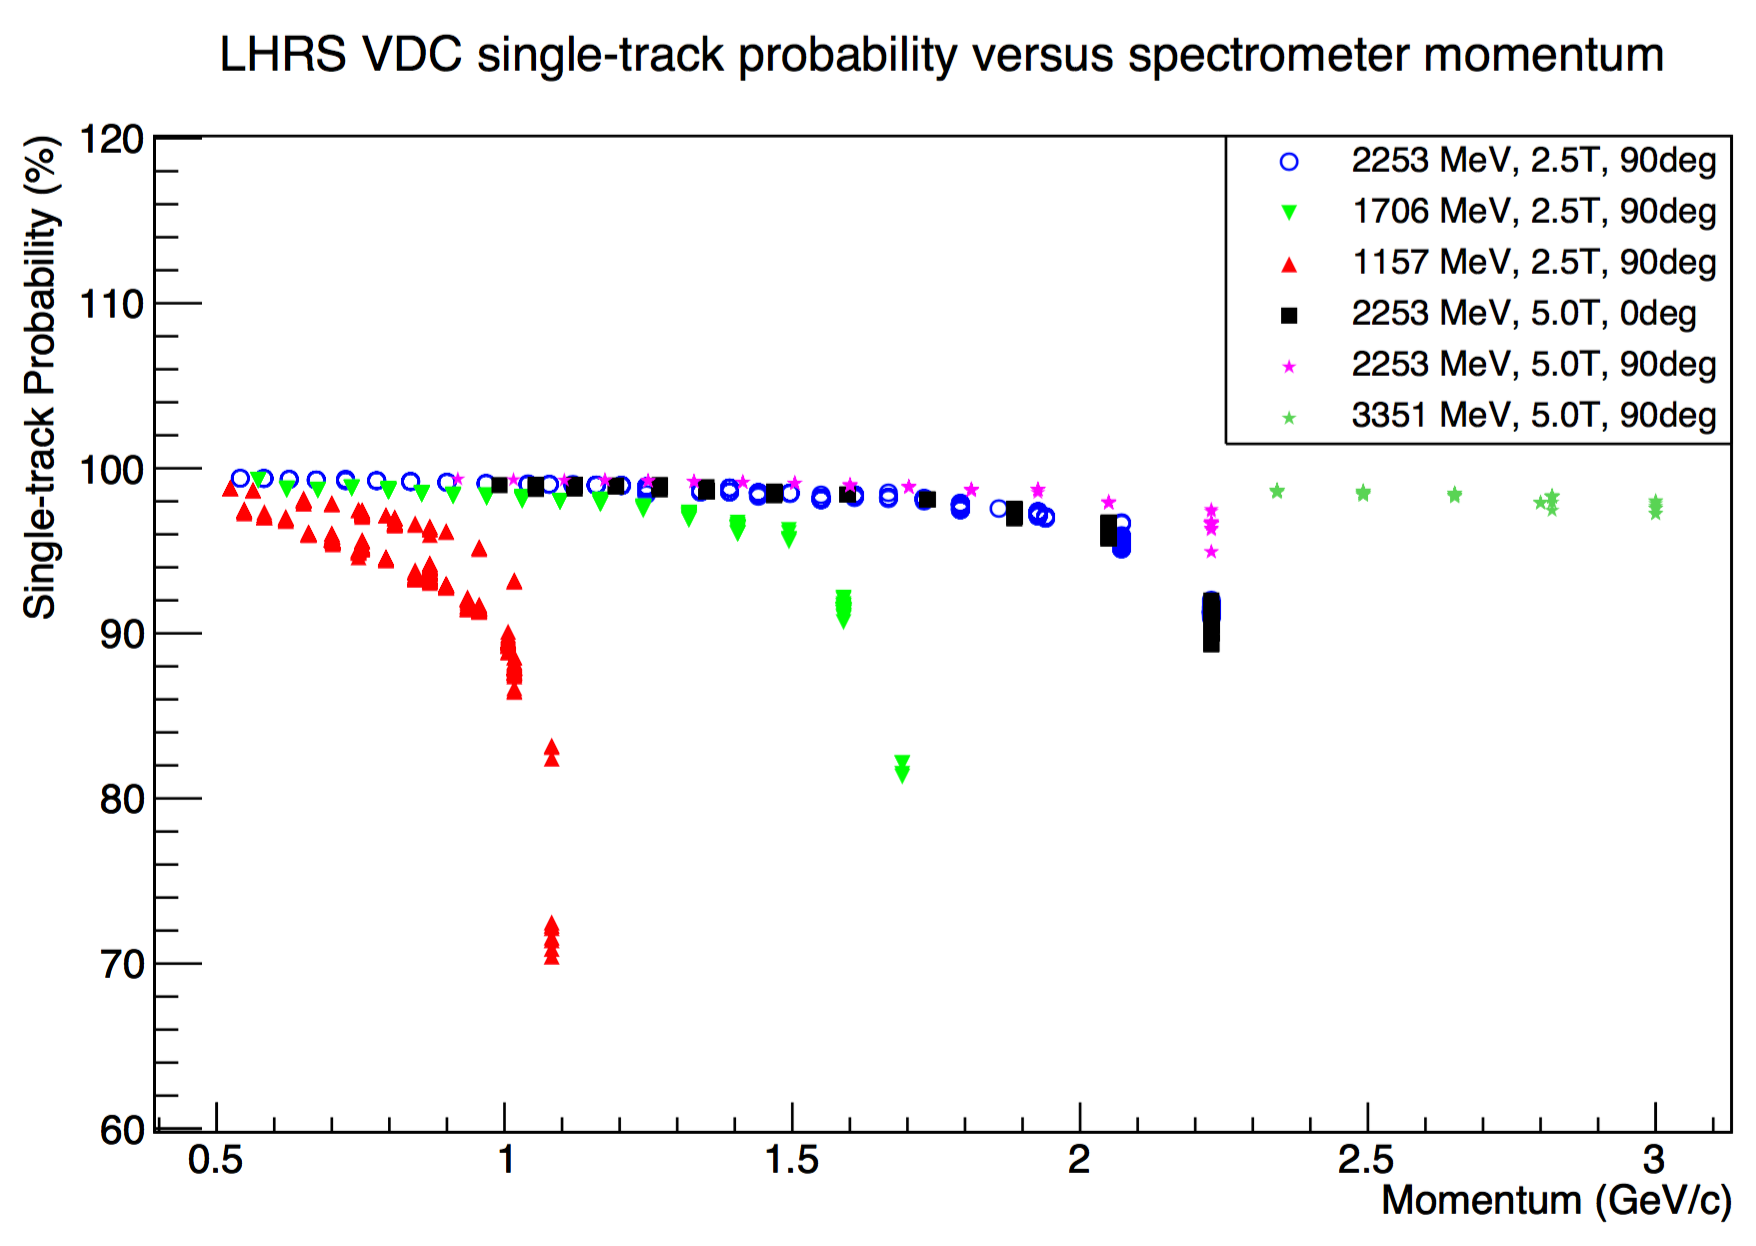
\includegraphics[width=\textwidth]{figs/single-track-left.png}
  \end{subfigure}
  \begin{subfigure}[t]{0.49\textwidth}
    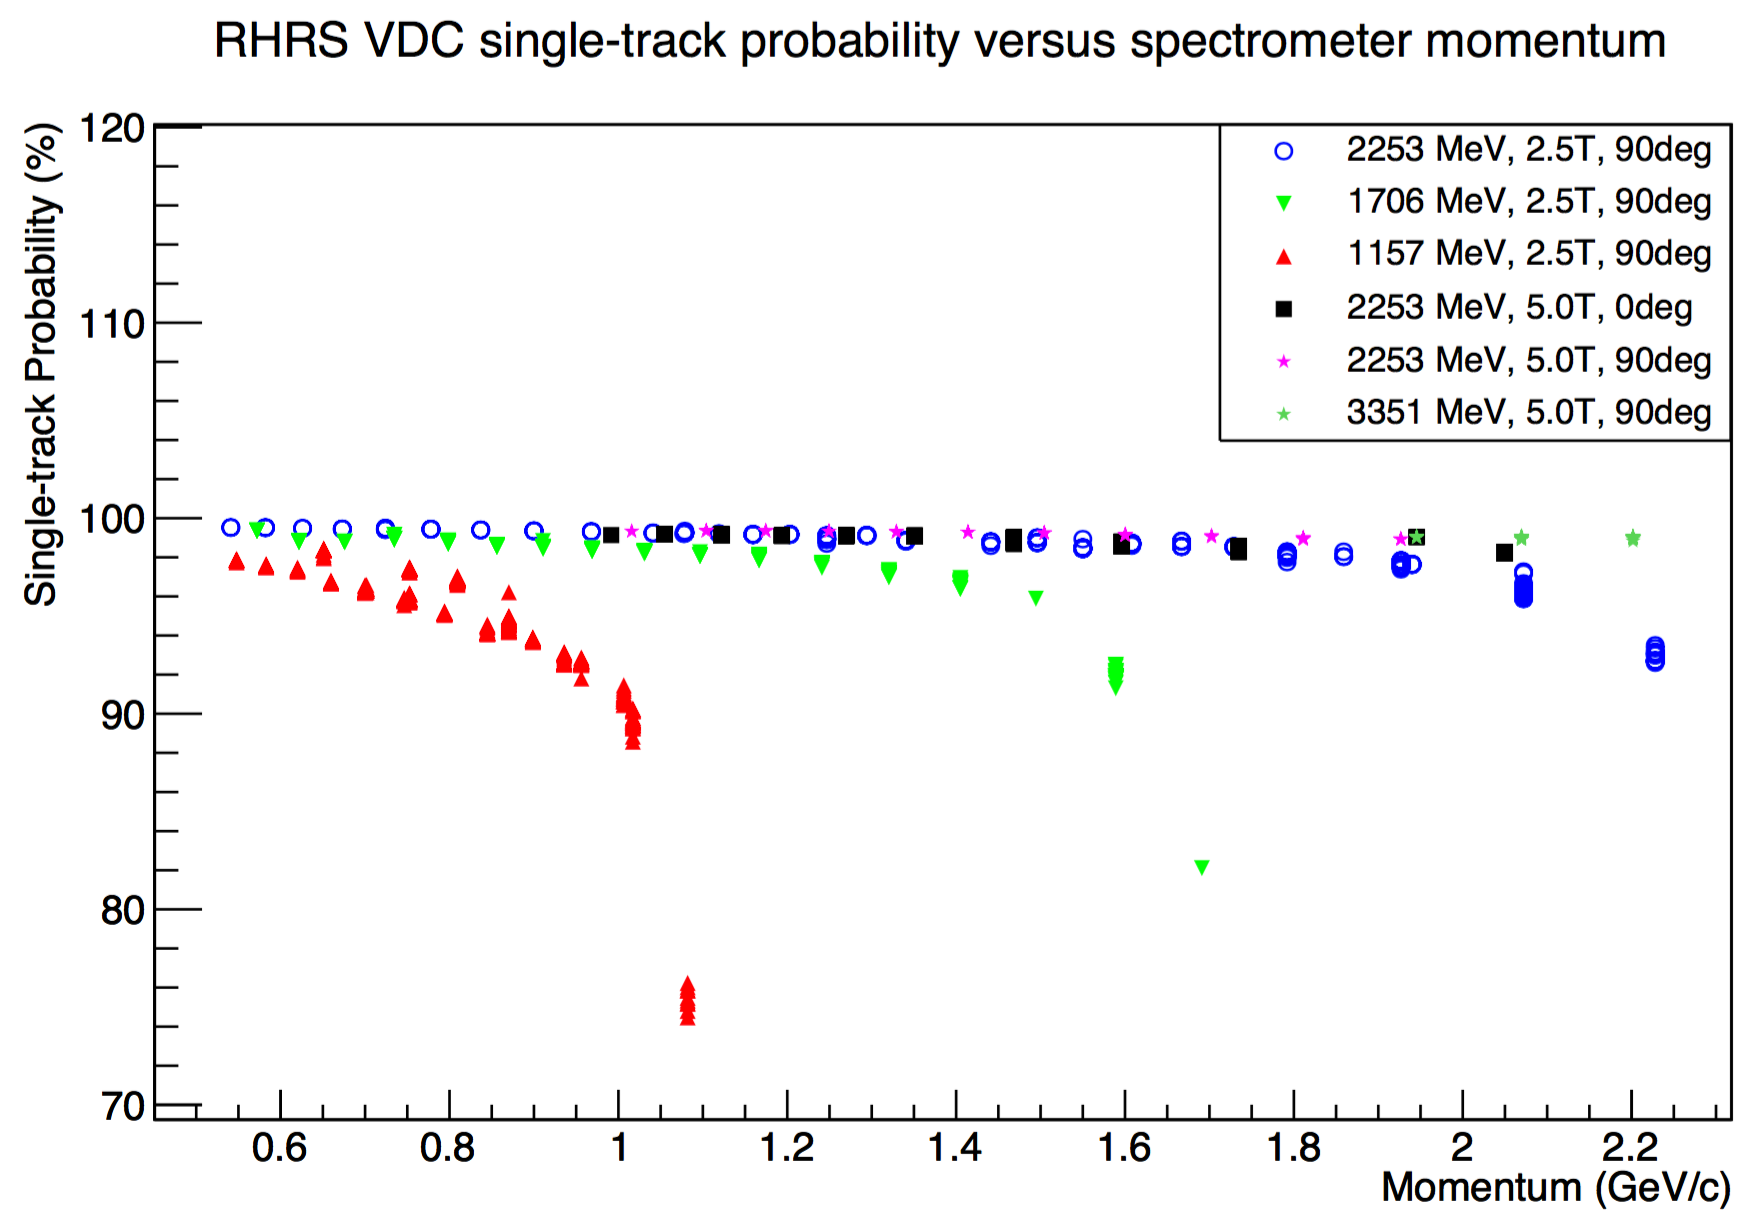
\includegraphics[width=\textwidth]{figs/single-track-right.png}
  \end{subfigure}
  \caption[Probability of an event leaving only one track in the VDC.]{Probability of an event leaving only one track in the VDC. Plot reproduced from \cite{Liu2013}. \label{C7S2F1}}
\end{figure}

The energy deposited in the calorimeters for each track is examined carefully to determine whether there is at least one good track reconstructed by VDC for each multi-track event. We can expect a multi-track event to have at least one good track if the energy deposited by one of the tracks in this event is larger than the central momentum of the spectrometer. After careful examination of multi-track events, the uncertainty of the VDC efficiency has been reduced to $<1$\% for most kinematic settings. \Cref{C7S2F2} gives the total VDC efficiency with the uncertainty for both arms of HRS. For most of the kinematic settings, the VDC efficiency is approximately 100\%. See Ref. \cite{Liu2013} for more detail of the multi-track efficiency analysis.

\begin{figure}[tb!]
  \centering
  \begin{subfigure}[t]{0.49\textwidth}
    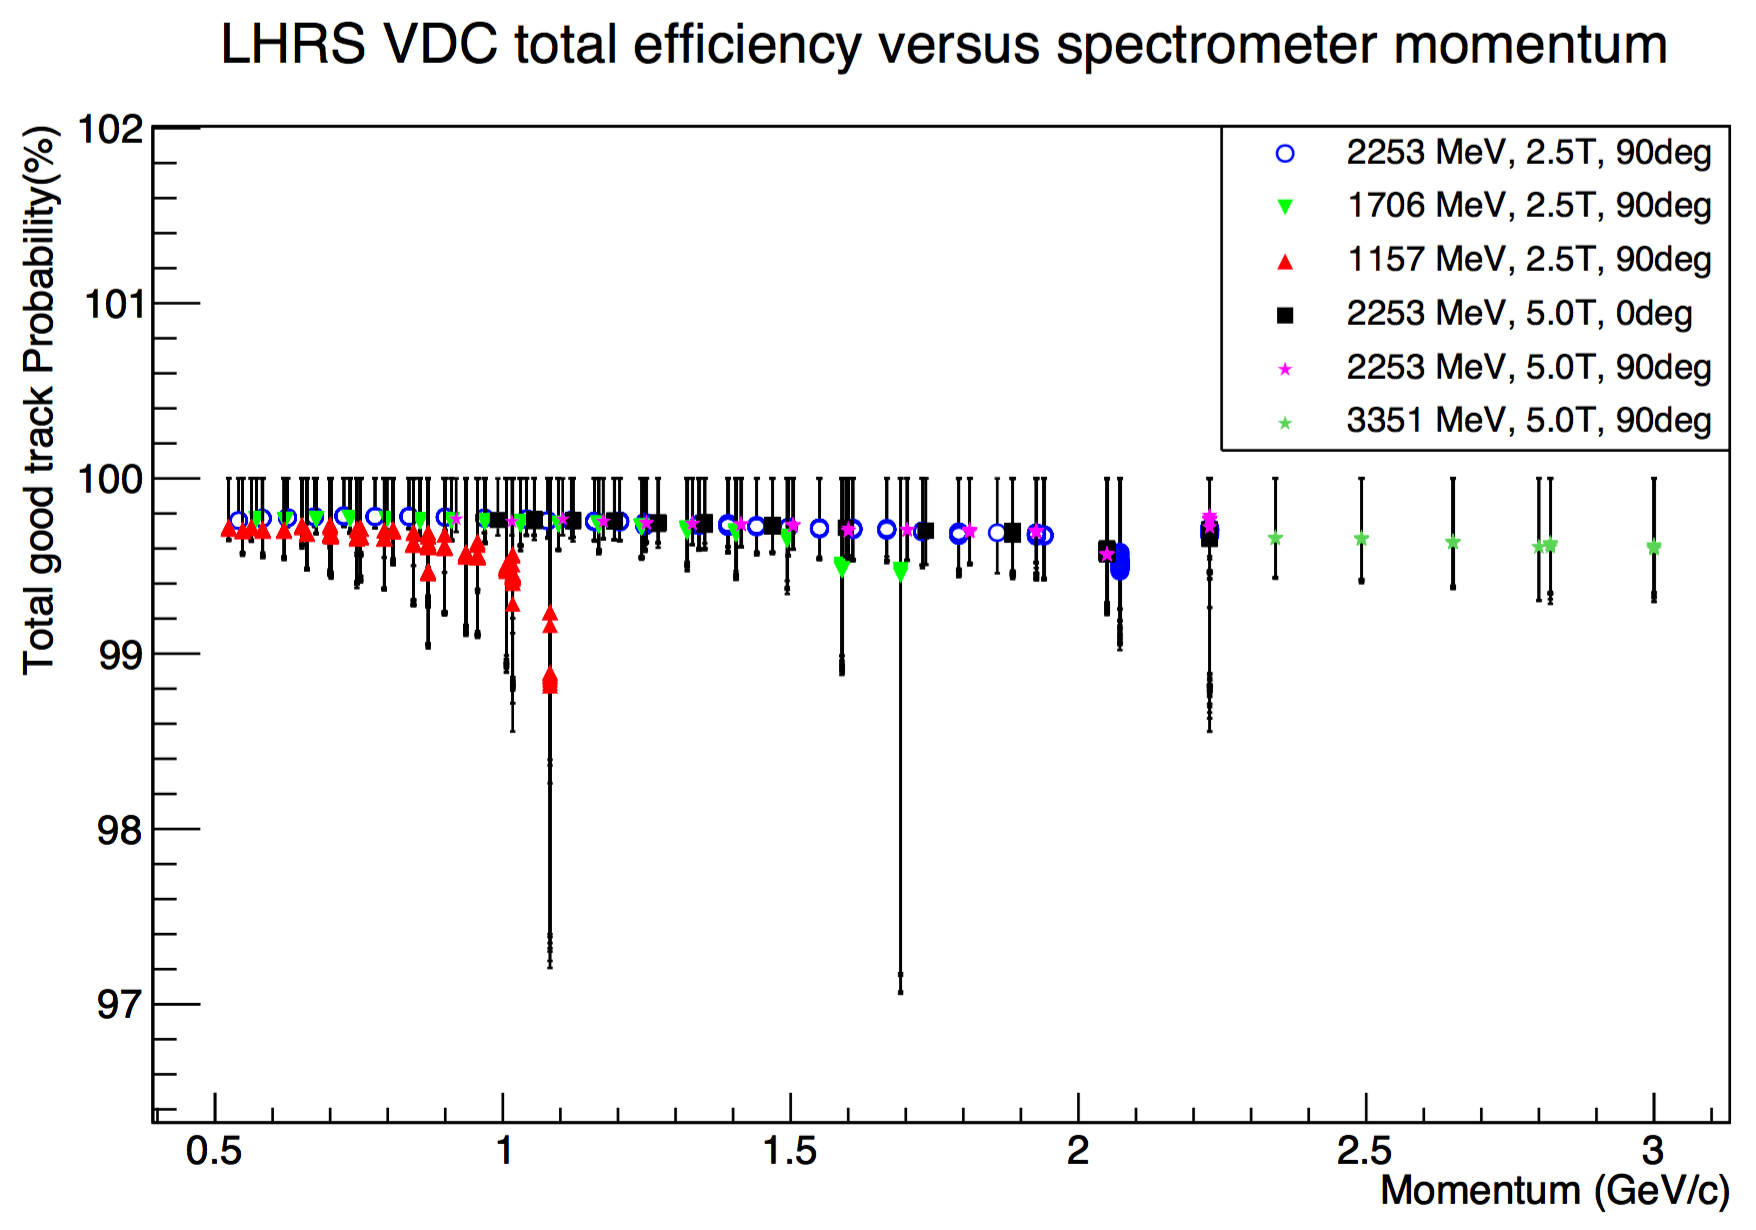
\includegraphics[width=\textwidth]{figs/VDC-efficiency-left.png}
  \end{subfigure}
  \begin{subfigure}[t]{0.49\textwidth}
    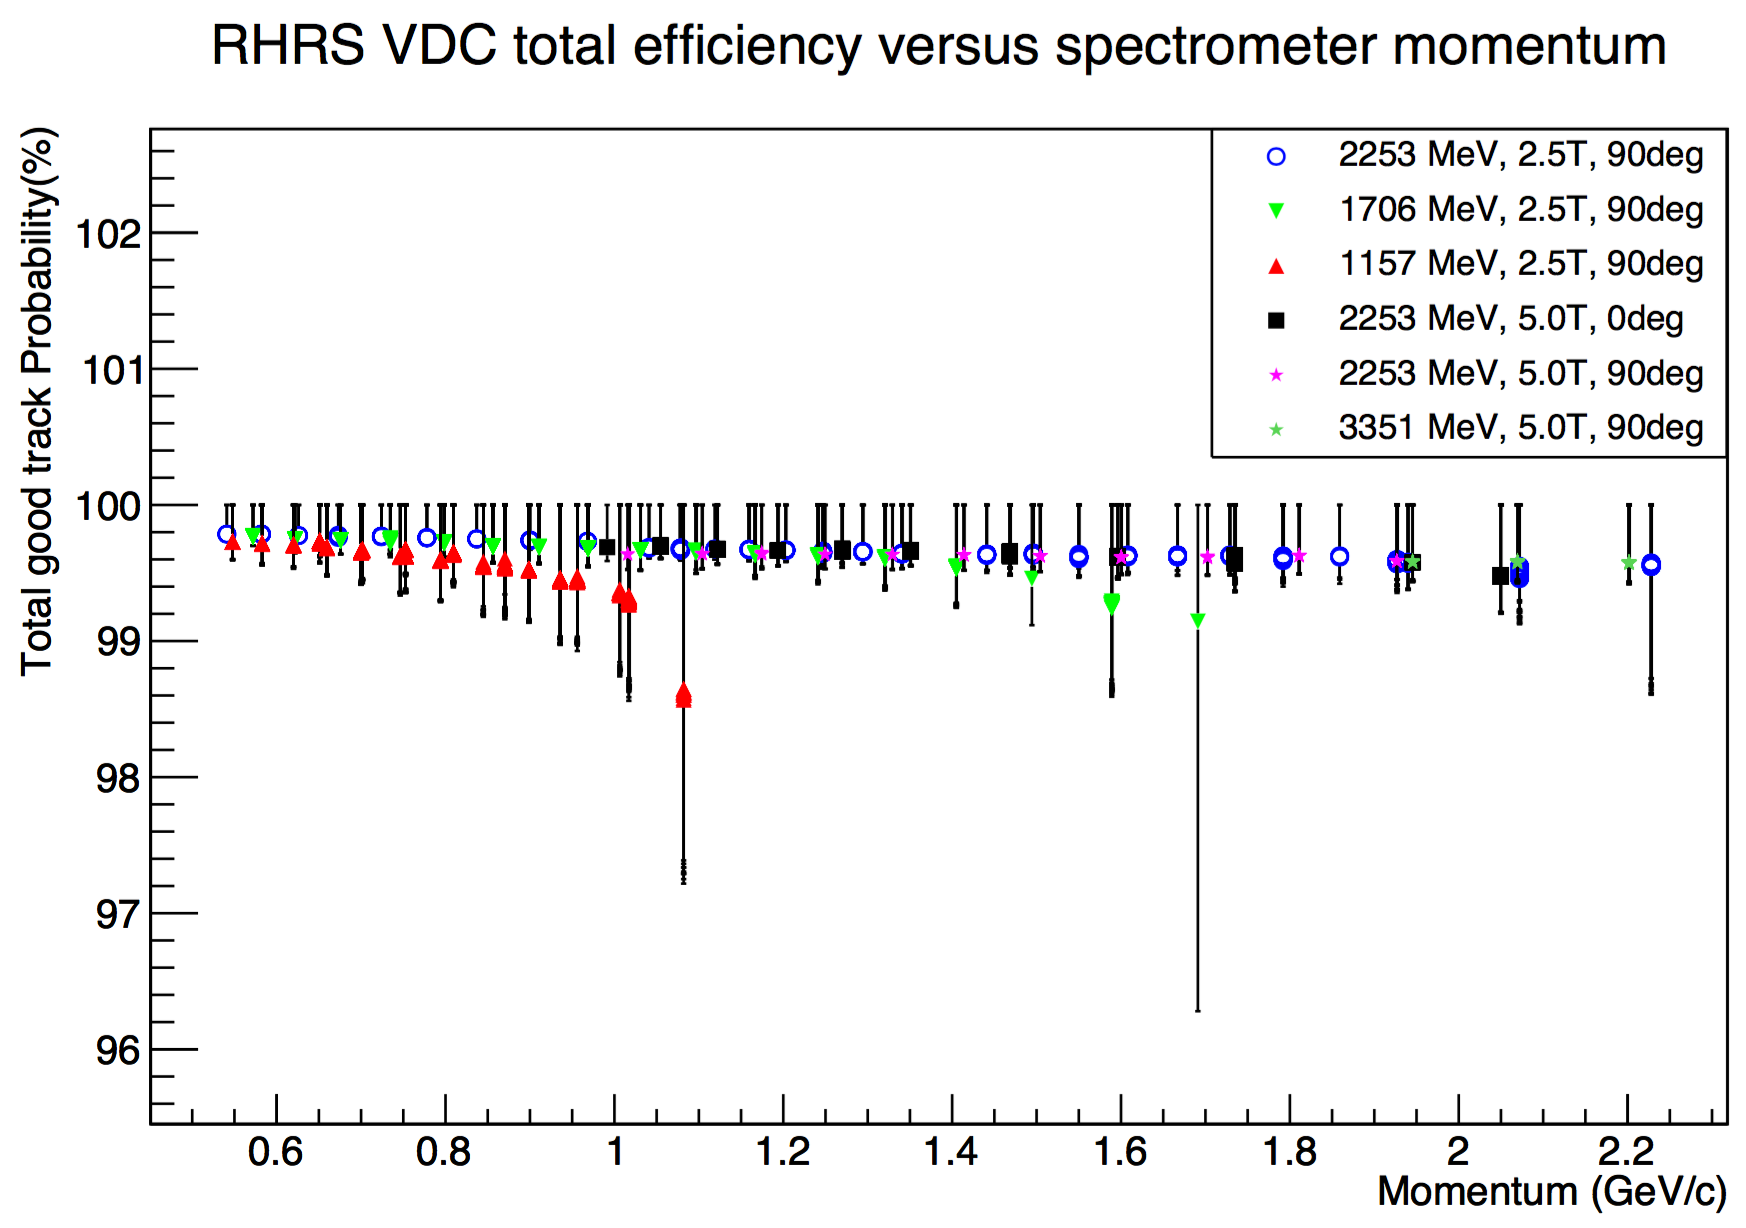
\includegraphics[width=\textwidth]{figs/VDC-efficiency-right.png}
  \end{subfigure}
  \caption[Total VDC efficiency.]{Total VDC efficiency. Plot reproduced from \cite{Liu2013}. \label{C7S2F2}}
\end{figure}

\subsection{Particle Identification Efficiency}
\label{C7S2SS2}

The Cherenkov detector and the electromagnetic calorimeter detectors of the HRS detector package are used to do particle identification (PID). All particles with the correct momentum-to-charge ratio are selected by the spectrometer, which include electrons, pions, kaons and etc. To ensure a good electron sample, cuts were applied to the data to select a clean electron sample. In the kinematics of E08-027, the major contamination arises from the pions. The majority of pions can be removed with a cut on the Cherenkov, since pions cannot directly trigger this detector as we explained in \Cref{C5S4SS2}. In practice, the gas Cherenkov cut is used together with two additional cuts: a cut on the first layer of the lead-glass calorimeter and a cut on the total energy deposited in the calorimeter. All three PID cuts are chosen to maximize the pion suppression while minimizing the removal of good electron events from the data sample.

\begin{figure}[tb!]
  \centering
  \begin{subfigure}[t]{0.49\textwidth}
    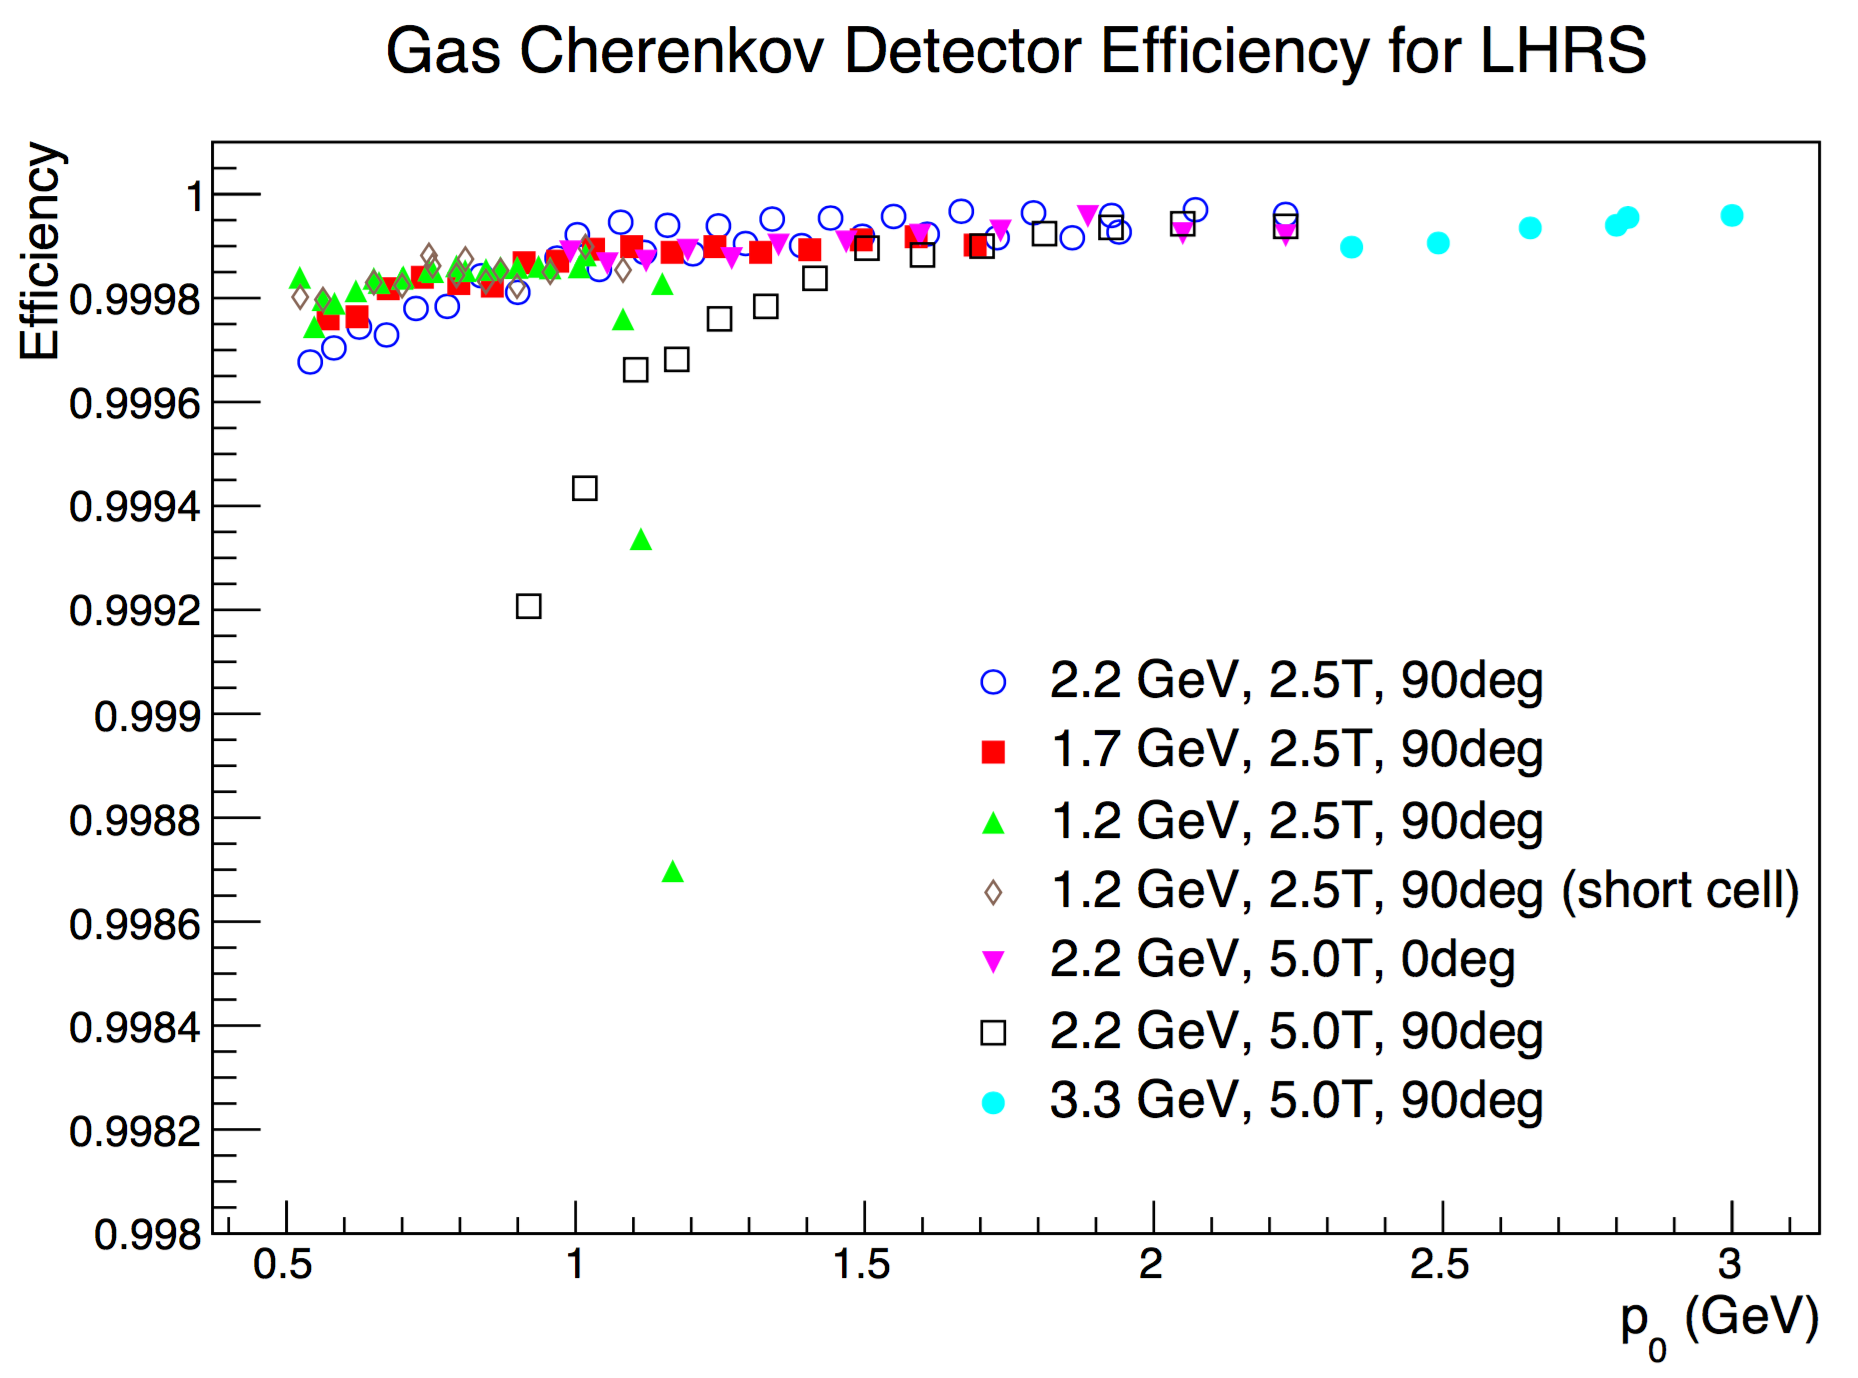
\includegraphics[width=\textwidth]{figs/Cherenkov-efficiency-left.png}
  \end{subfigure}
  \begin{subfigure}[t]{0.49\textwidth}
    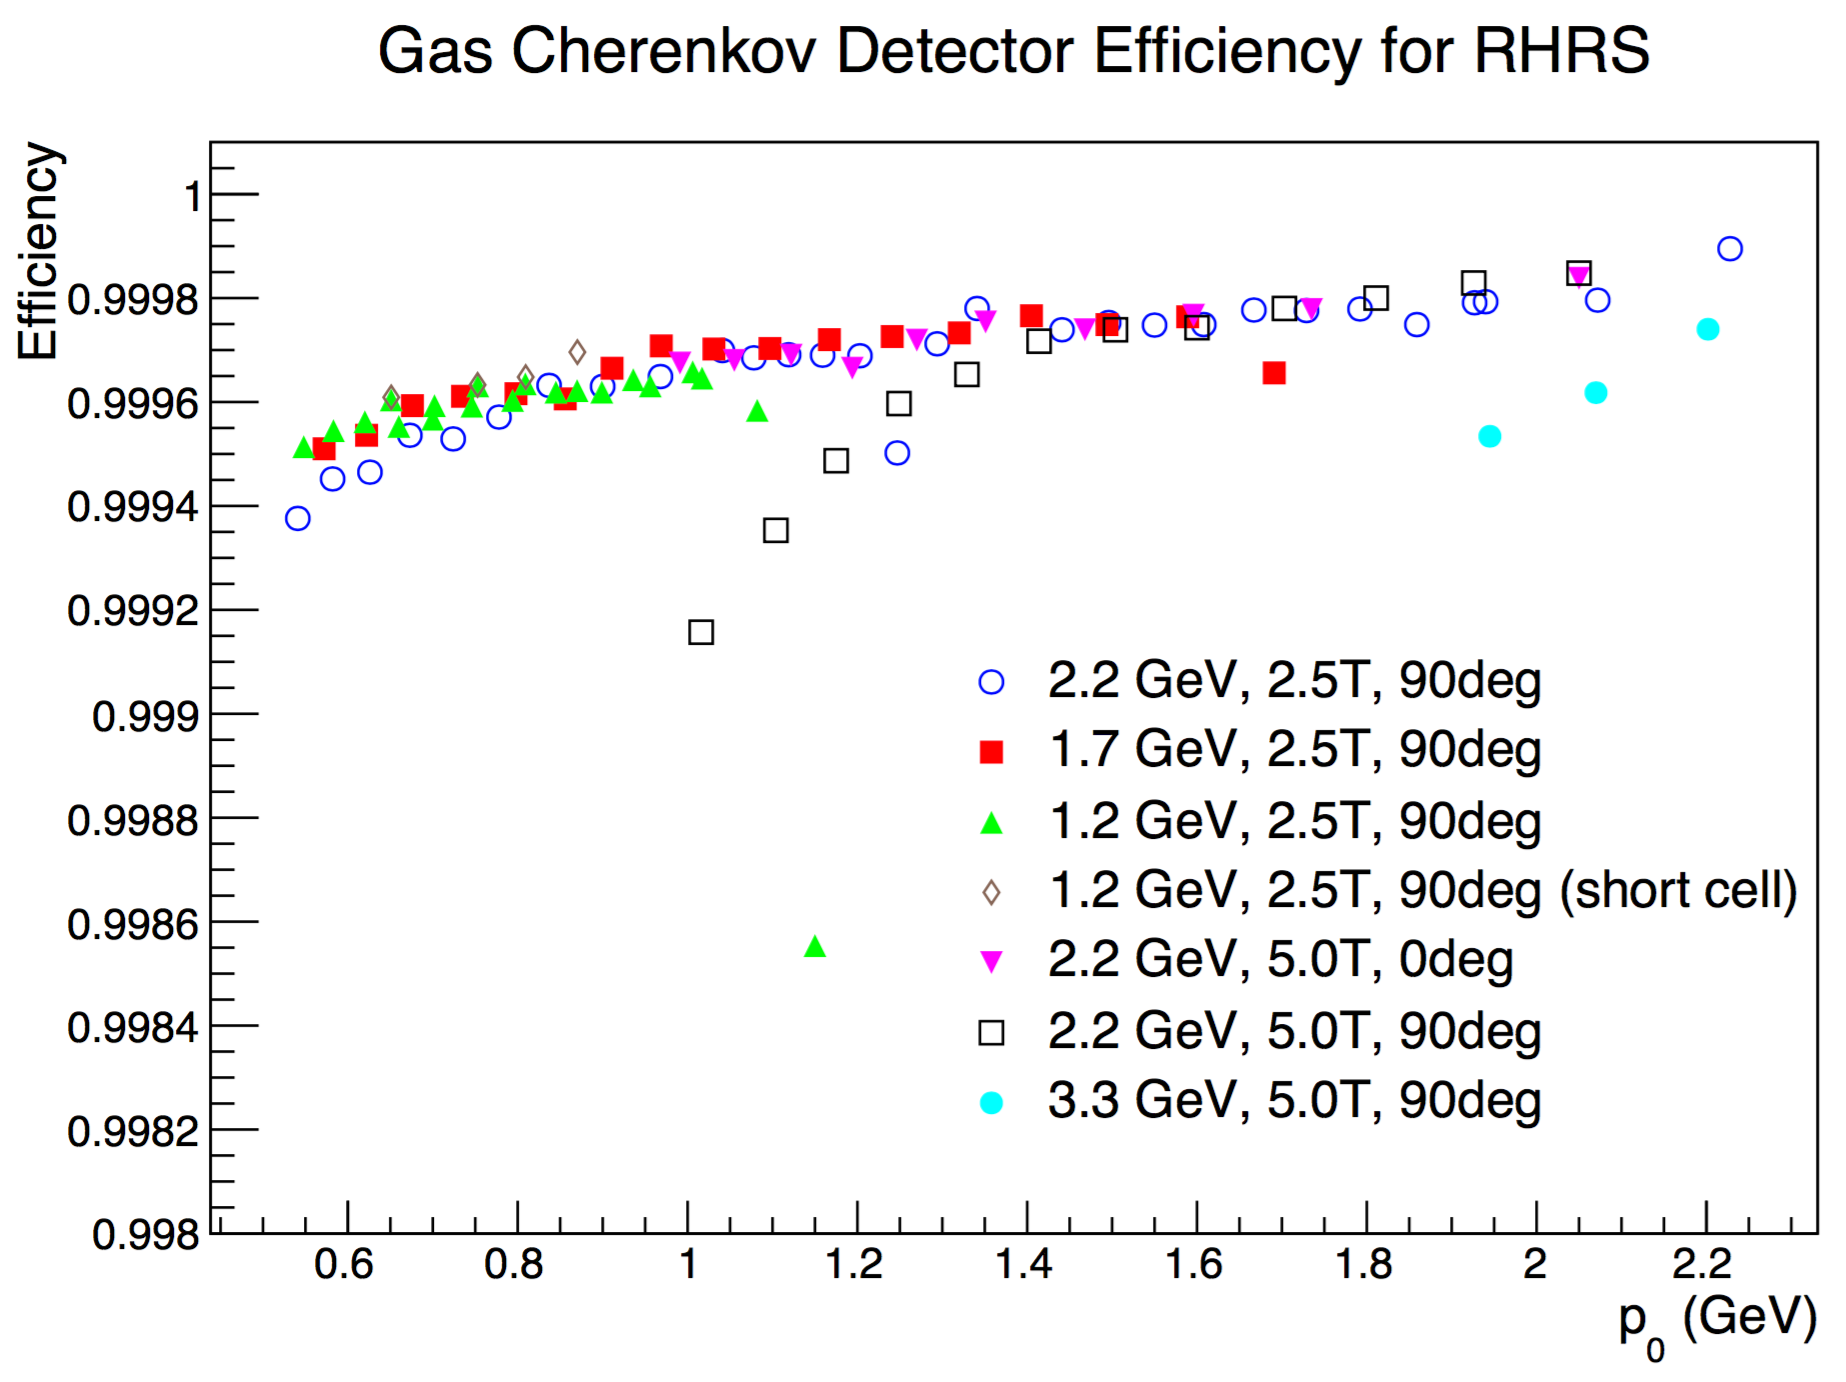
\includegraphics[width=\textwidth]{figs/Cherenkov-efficiency-right.png}
  \end{subfigure}
  \caption[Detector efficiencies of the gas Cherenkov detectors.]{Detector efficiencies of the gas Cherenkov detectors. Plot reproduced from \cite{Cummings2013}. \label{C7S2F3}}
\end{figure}

\begin{figure}[tb!]
  \centering
  \begin{subfigure}[t]{0.49\textwidth}
    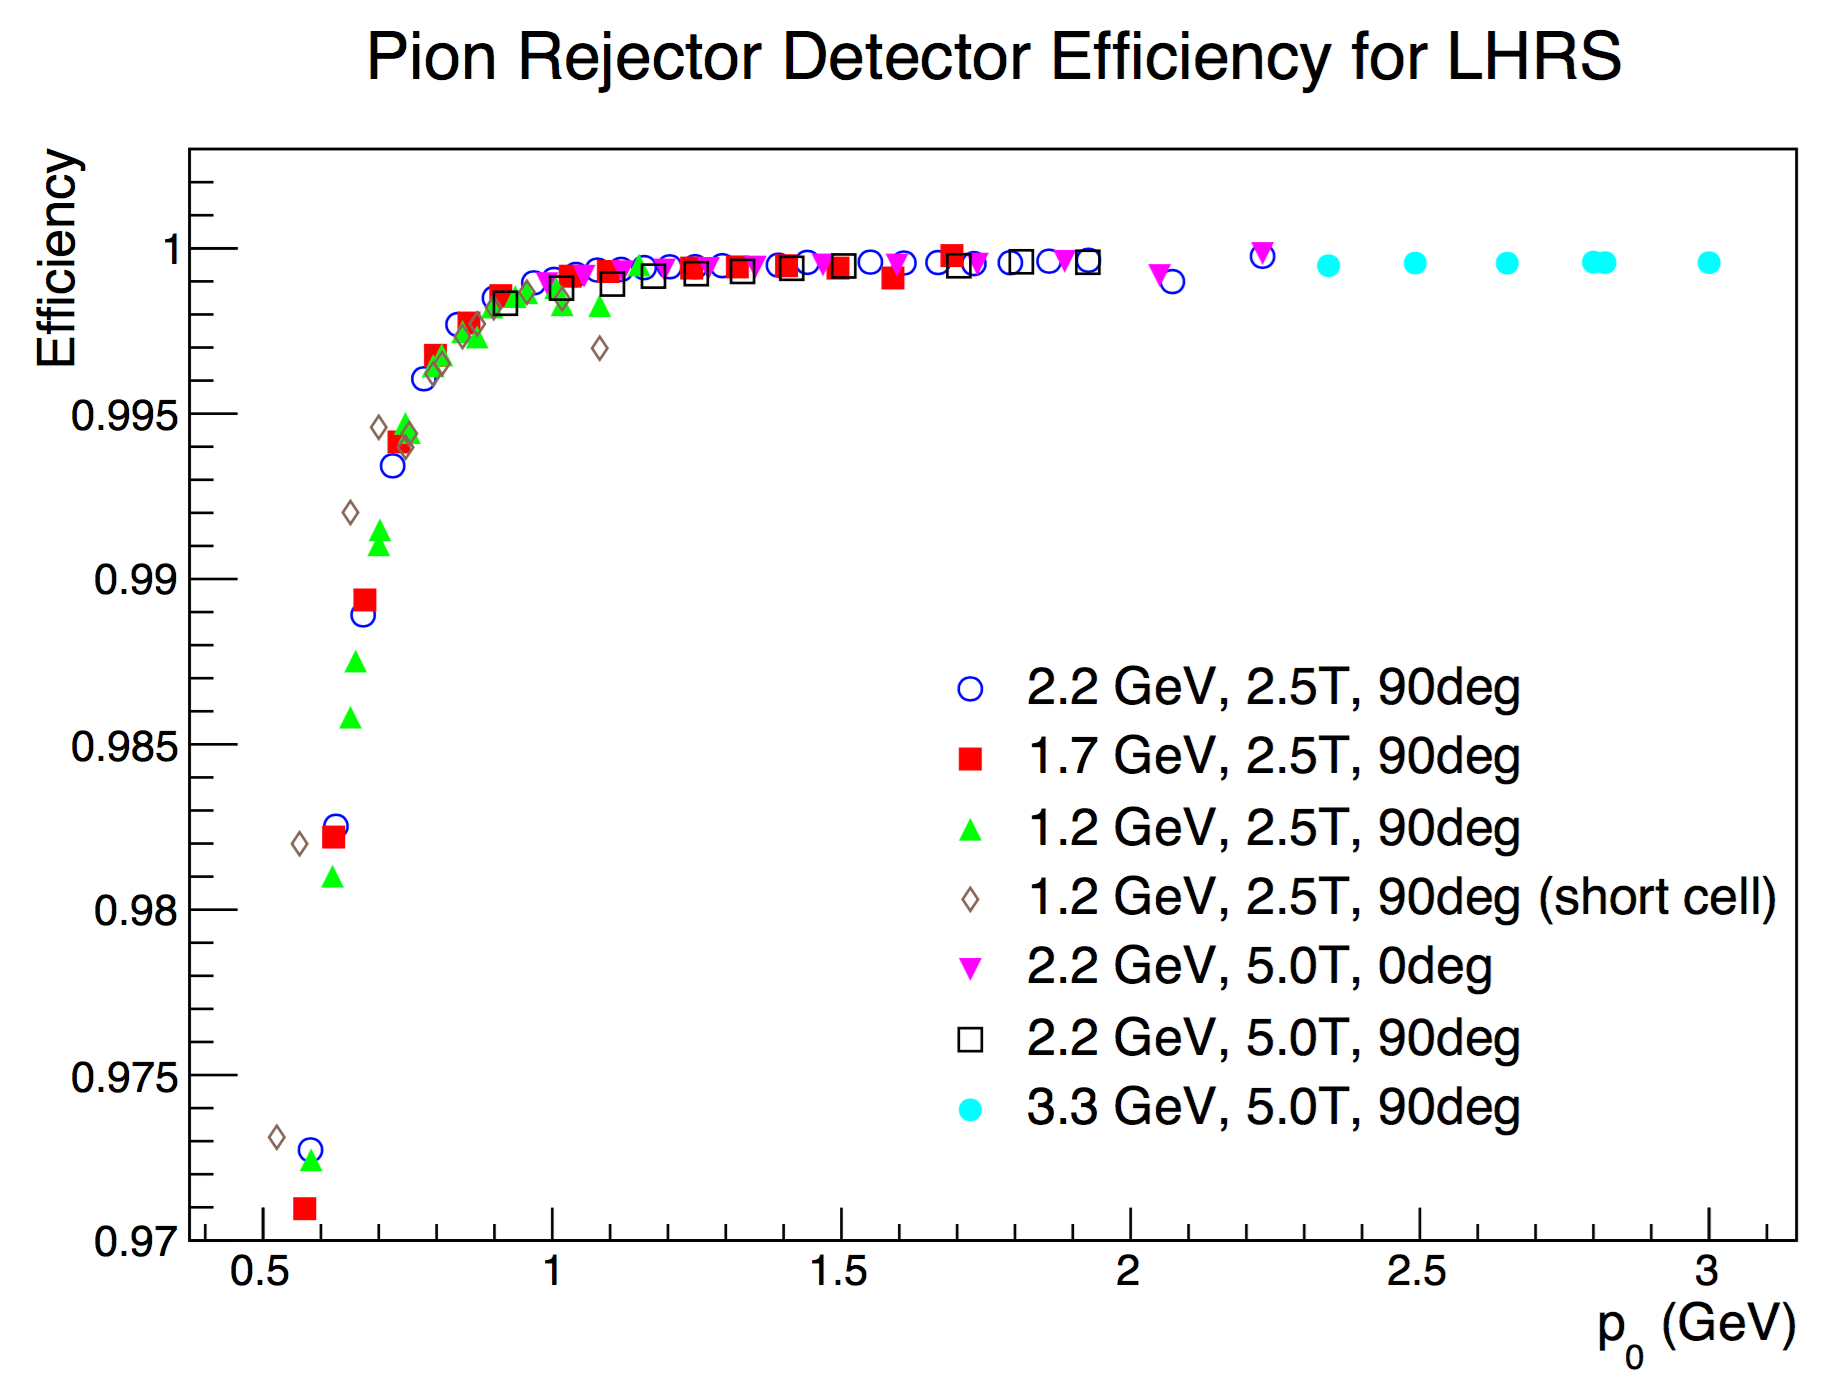
\includegraphics[width=\textwidth]{figs/calorimeters-efficiency-left.png}
  \end{subfigure}
  \begin{subfigure}[t]{0.49\textwidth}
    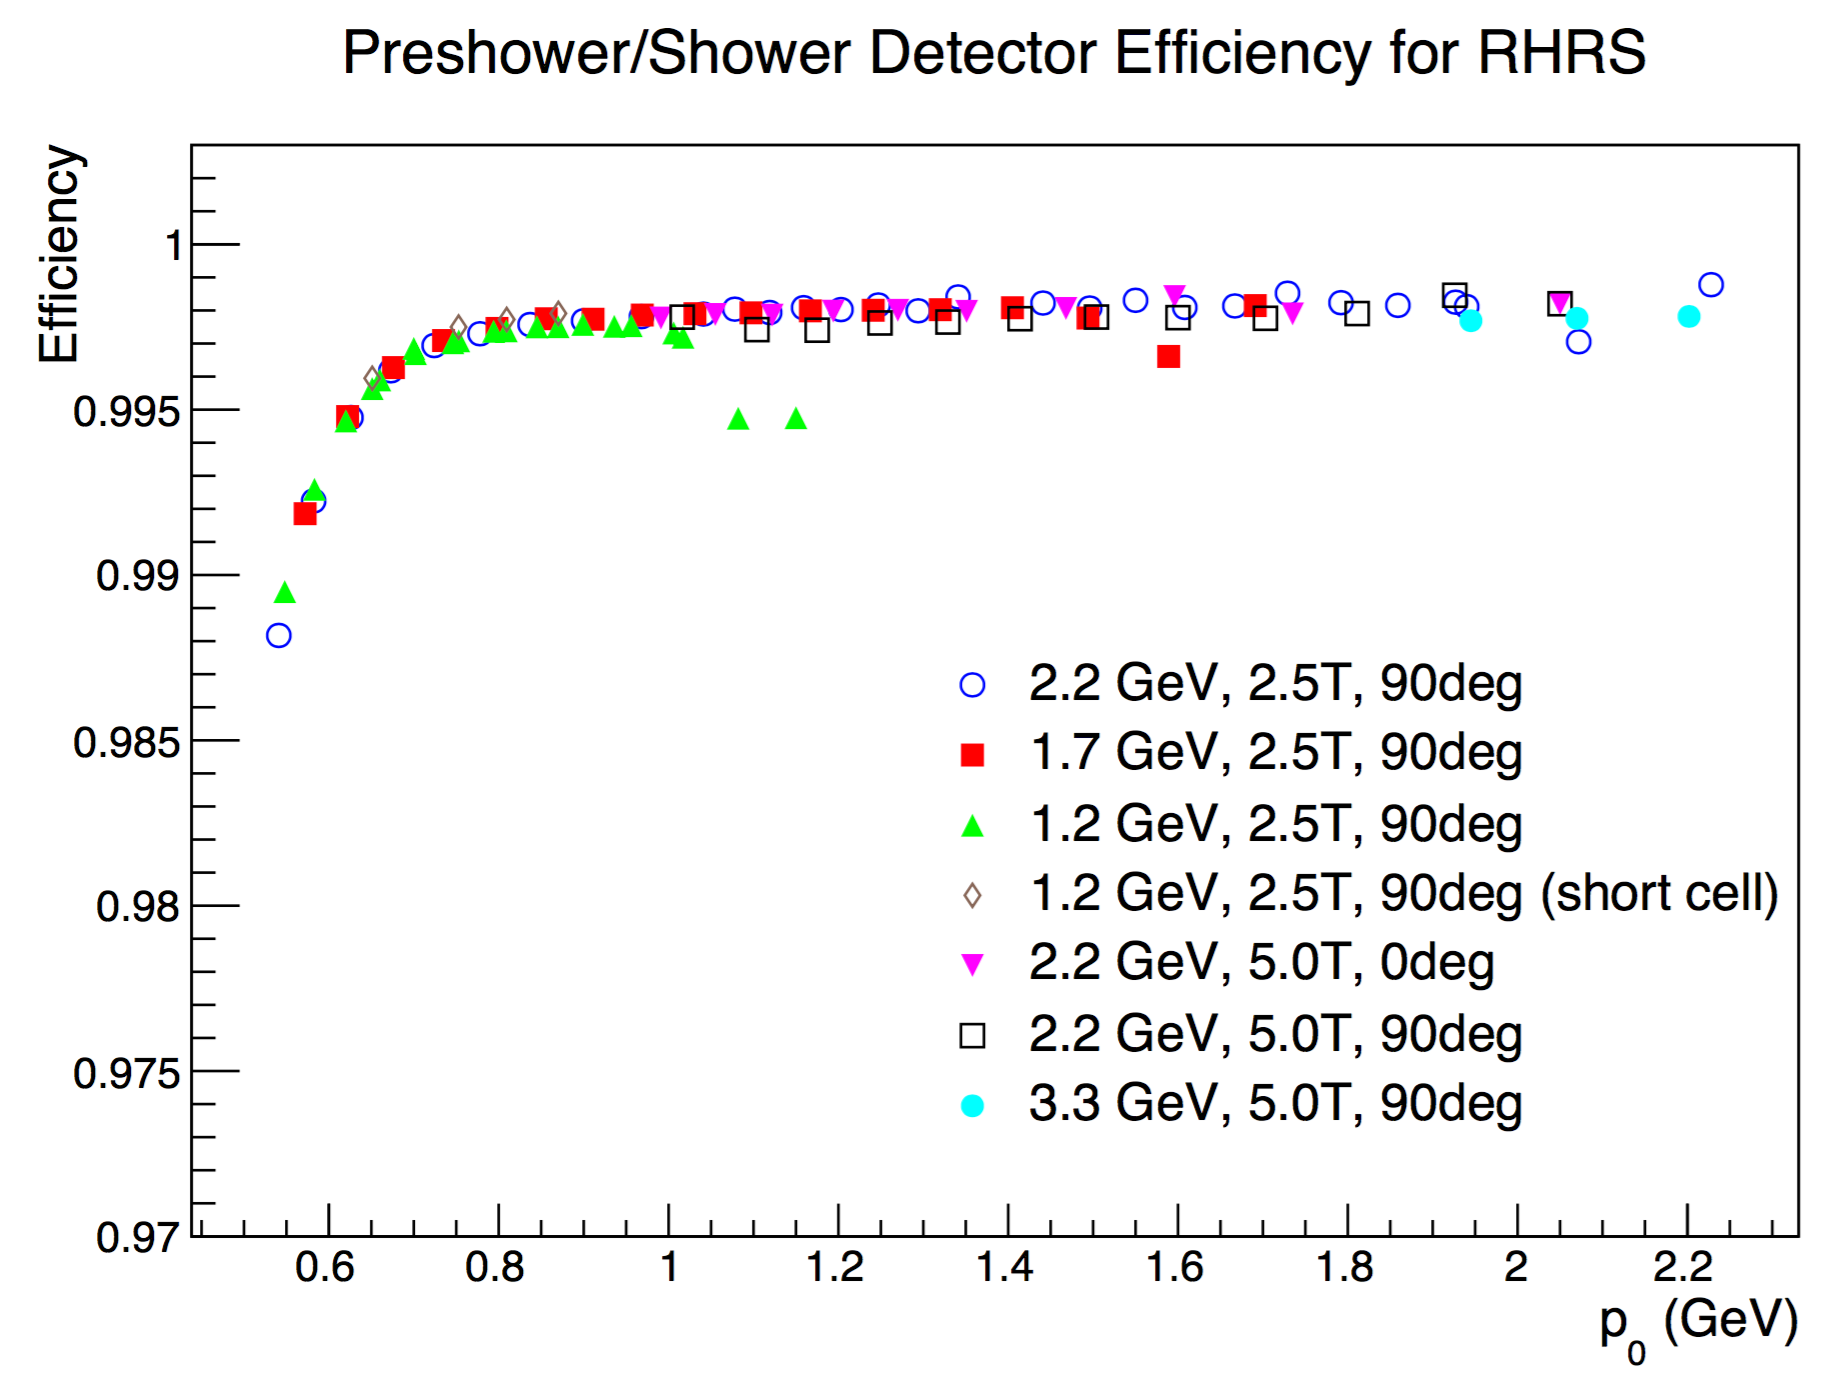
\includegraphics[width=\textwidth]{figs/calorimeters-efficiency-right.png}
  \end{subfigure}
  \caption[Detector efficiencies of the electromagnetic calorimeters.]{Detector efficiencies of the electromagnetic calorimeters. Plot reproduced from \cite{Cummings2013}. \label{C7S2F4}}
\end{figure}

The detector performance results for the Cherenkov detector and the calorimeters are discussed in details in Ref. \cite{Cummings2013}, and are briefly summarized here. The detector efficiencies of the gas Cherenkov detectors are shown in \Cref{C7S2F3}. The efficiency of the gas Cherenkov detector for both arms of the HRS is found to be above 99.8\% across the entire range of kinematics. \Cref{C7S2F4} also shows the detector efficiencies of the electromagnetic calorimeters for the left and right arm of the HRS. The detection efficiency of the pion rejectors in HRS-L is above 98\%, the efficiency of the pre-shower and shower in HRS-R is above 98.8\% for all kinematic settings. These results indicate that the performance of the PID detectors is very good during the experiment.

The gas Cherenkov cut works as a threshold cut on both arms, which is a constant cut for every kinematic setting. The calorimeter cuts are then chosen to keep the overall electron detection efficiency above 99\%. A conservative cut is placed on the pre-shower for HRS-R, and a separate cut is placed on the total deposited energy; these cuts are momentum dependent unlike the gas Cherenkov cuts. For HRS-L, the cut on the first layer does not need to be as conservative, since more energy is deposited in the first layer of the pion rejector which is thicker than the pre-shower in right arm. Ref. \cite{Cummings2013} also discussed the pion suppression efficiencies in detail. After PID cuts are applied, the level of residual pion contamination is very low, with $\pi/e<0.0052$ for all kinematic settings on both arms of the HRS, as shown in \Cref{C7S2F5}.

\begin{figure}[tb!]
  \centering
  \begin{subfigure}[t]{0.49\textwidth}
    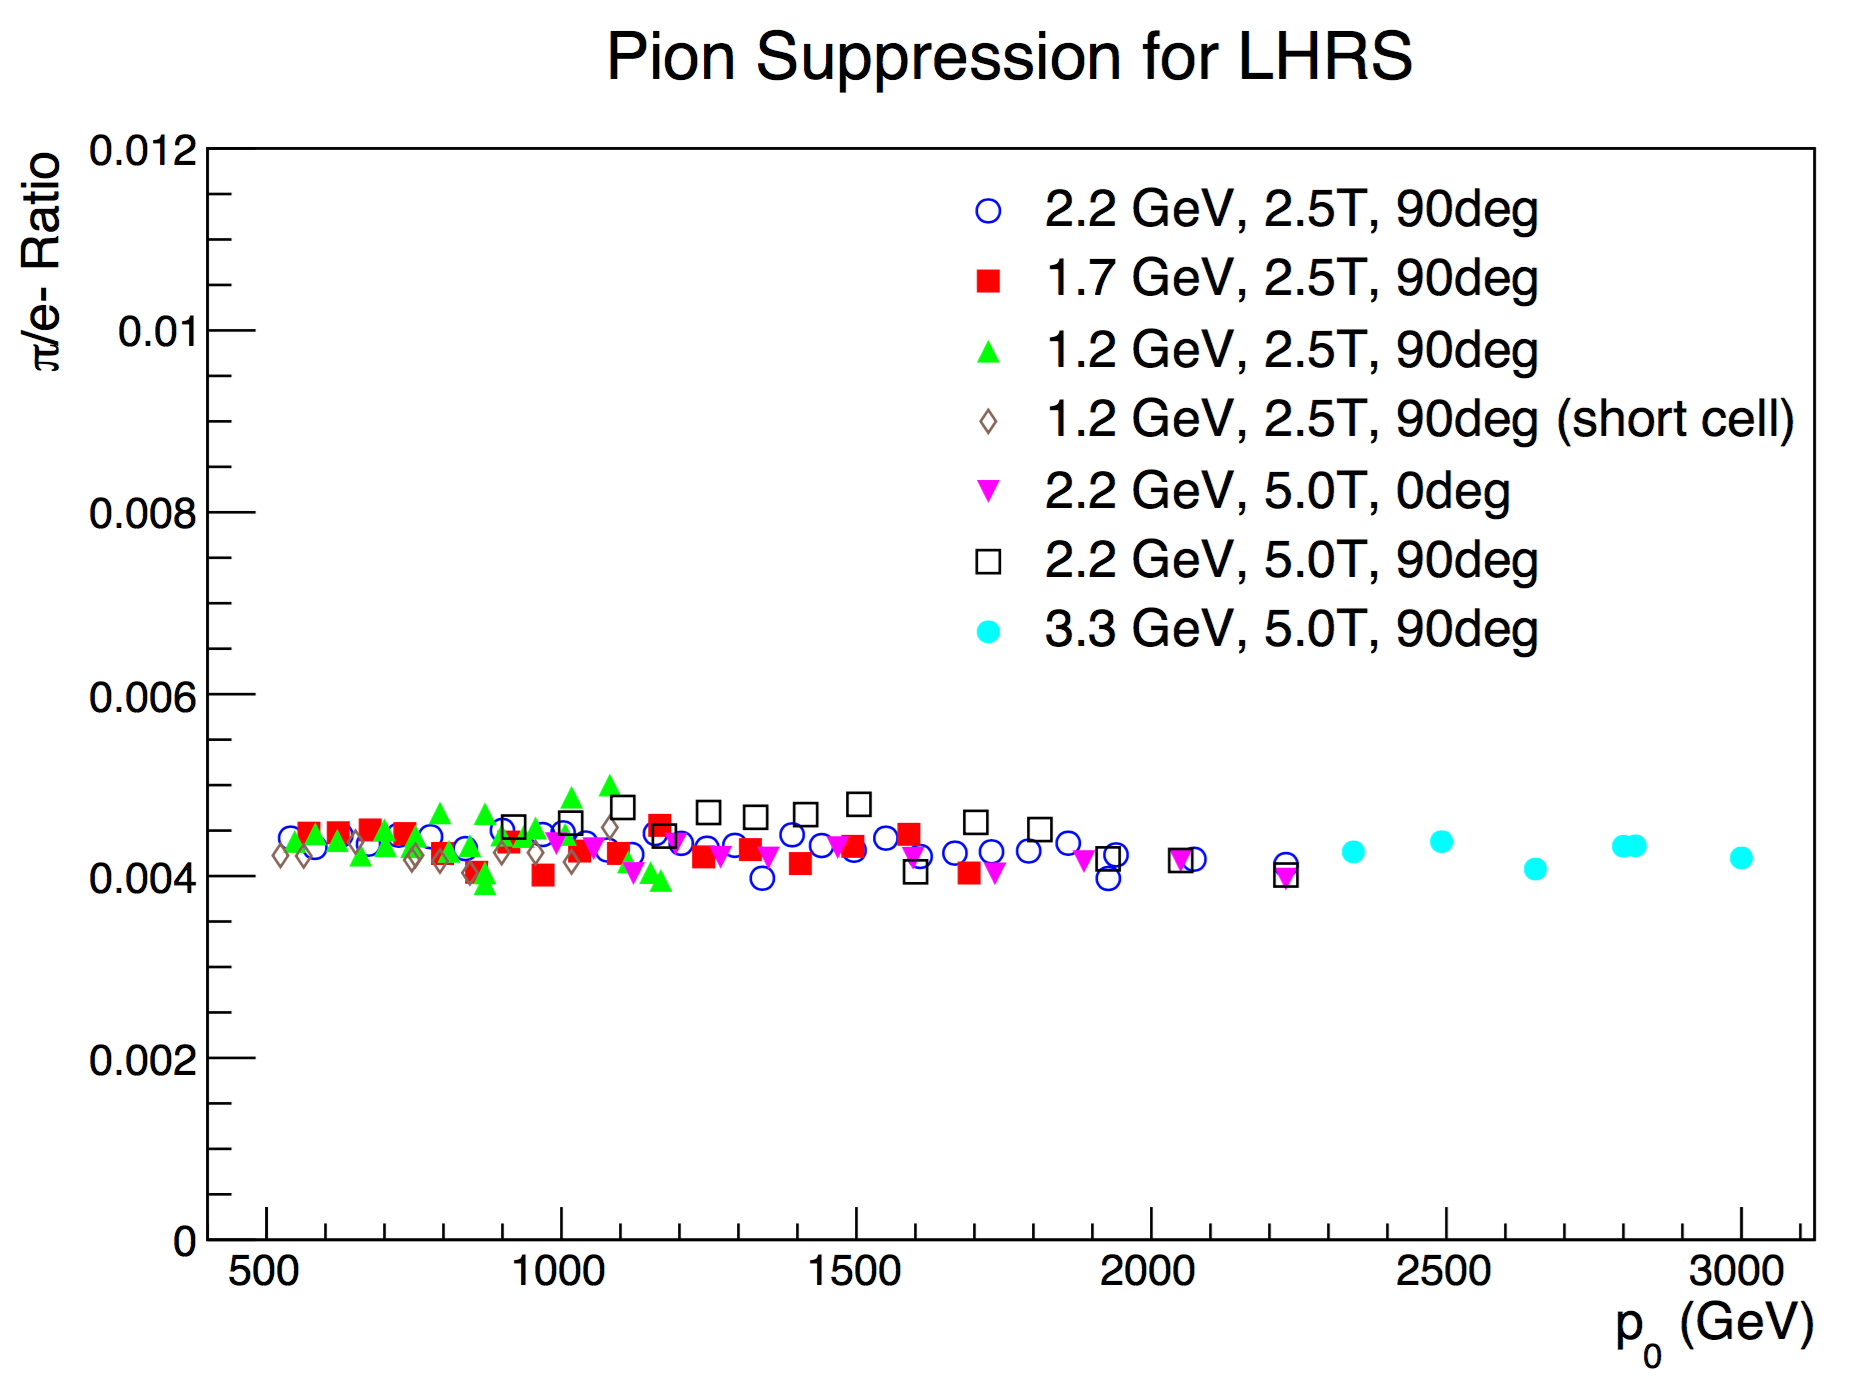
\includegraphics[width=\textwidth]{figs/pion-suppression-left.png}
  \end{subfigure}
  \begin{subfigure}[t]{0.49\textwidth}
    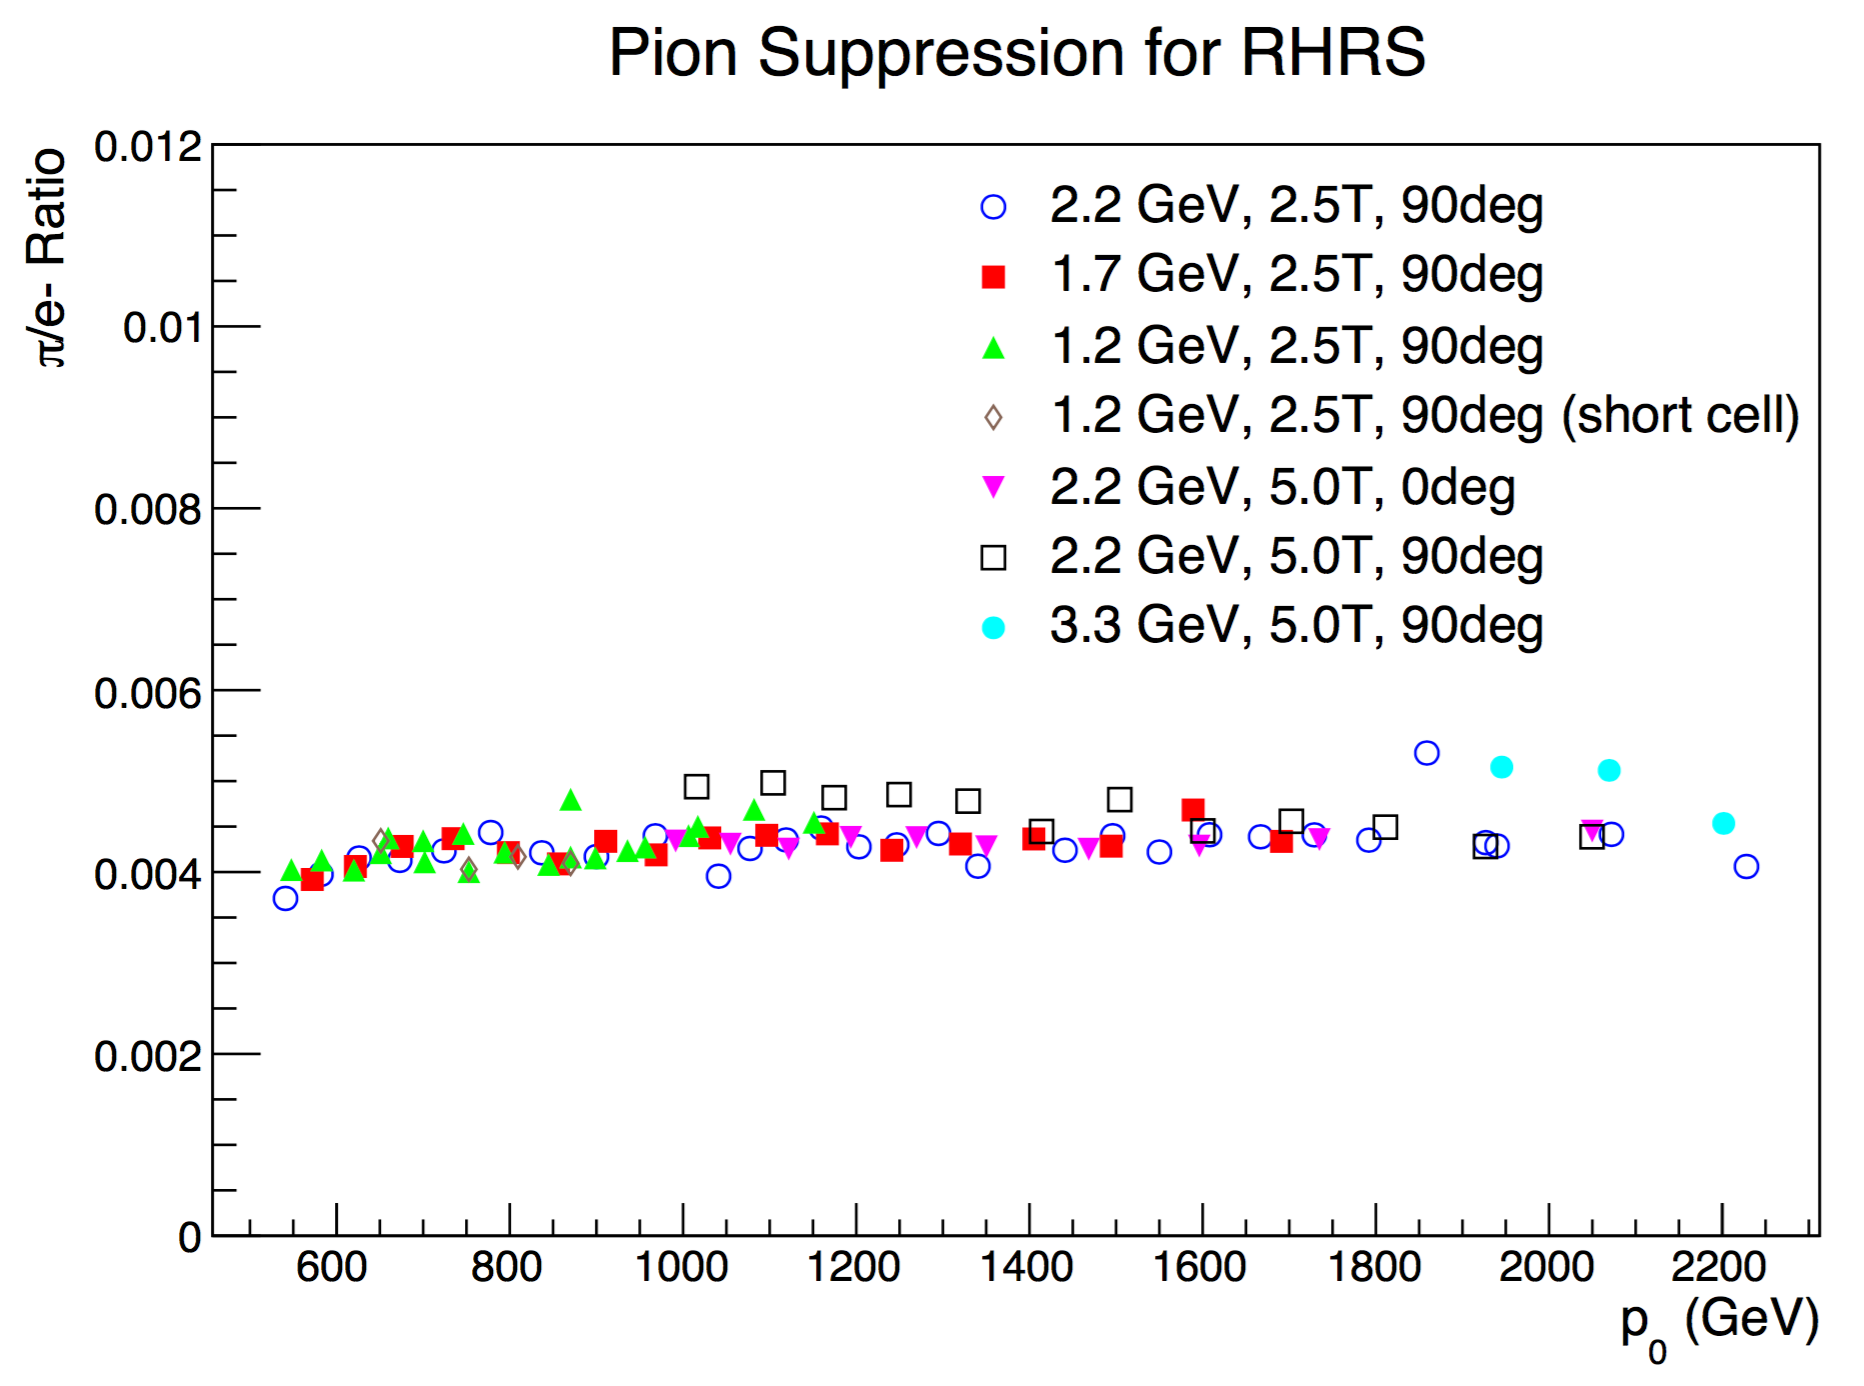
\includegraphics[width=\textwidth]{figs/pion-suppression-right.png}
  \end{subfigure}
  \caption[Residual pion contamination after PID cuts are applied.]{Residual pion contamination after PID cuts are applied. Plot reproduced from \cite{Cummings2013}. \label{C7S2F5}}
\end{figure}

\section{Packing Fraction Analysis}
\label{C7S3}

Ideally the target cell should be completely filled with solid ammonia. However, due to the size and shape of the ammonia beads, there is some space between the beads and this space is filled with liquid helium. The packing fraction is defined as the effective length of the ammonia divided by the total length of the target. During the experiment, data is collected with the production NH${}_3$ target and the dummy target which has been described in \Cref{C5S3SS2}. These data are used to extract the packing fraction.

The normalized yield for each run is defined as:
\begin{equation} \label{C7S3E1}
Y = \frac{ps\cdot N}{Q\cdot LT\cdot \eta_{\mathrm{det}}}.
\end{equation}
Here the definitions of each quantity are exactly the same as \cref{C7S1E6}. Using the packing fraction $p_f$, the yield of a production run could be broken into contributions of each target materials:
\begin{equation} \label{C7S3E2}
Y_{\mathrm{target}} = Y_{\mathrm{He}}^{\mathrm{out}}+(1-p_f)Y_{\mathrm{He}}^{\mathrm{cell}}+p_fY_{\mathrm{NH_{3}}}^{\mathrm{cell}},
\end{equation}
where the $Y_{\mathrm{He}}^{\mathrm{cell}}$ is the yield of a target cell full of liquid helium, the $Y_{\mathrm{He}}^{\mathrm{cell}}$ is the yield of a target cell with pure ammonia and the $Y_{\mathrm{He}}^{\mathrm{out}}$ is the yield from liquid helium inside the target nose, but outside the target cell.

The dummy target cell is identical to the ammonia cell except that it is filled with liquid helium but not NH${}_3$ beads. Thus the contributions from the liquid helium can be obtained from the yield $Y_{\mathrm{dummy}}$ of a run with dummy target. The $Y_{\mathrm{He}}^{\mathrm{cell}}$ and $Y_{\mathrm{He}}^{\mathrm{out}}$ can then be expressed in terms of $Y_{\mathrm{dummy}}$:
\begin{align} \label{C7S3E3}
Y_{\mathrm{He}}^{\mathrm{cell}} & = \left(\frac{L_{\mathrm{cell}}}{L_{\mathrm{total}}}\right)Y_{\mathrm{dummy}}, \\ \label{C7S3E4}
Y_{\mathrm{He}}^{\mathrm{out}} & = \left(\frac{L_{\mathrm{total}}-L_{\mathrm{cell}}}{L_{\mathrm{total}}}\right)Y_{\mathrm{dummy}},
\end{align}
where the $L_{\mathrm{cell}}$ is the length of the target cell and $L_{\mathrm{total}}$ is the effective total length of the target nose.

Thus the packing fraction can be expressed as:
\begin{equation} \label{C7S3E5}
p_f = \left(\frac{L_{\mathrm{total}}}{L_{\mathrm{cell}}}\right)\left(\frac{Y_{\mathrm{target}}}{Y_{\mathrm{dummy}}}-1\right)\left(\frac{Y_{\mathrm{NH_3}}^{\mathrm{cell}}}{Y_{\mathrm{He}}^{\mathrm{cell}}}-1\right)^{-1}.
\end{equation}
It is not possible to obtain the quantity $Y_{\mathrm{NH_3}}^{\mathrm{cell}}$ from the data. However, the ratio $Y_{\mathrm{NH_3}}^{\mathrm{cell}}/Y_{\mathrm{He}}^{\mathrm{cell}}$ could be expressed in terms of the cross-sections since the yield can be expressed as:
\begin{equation} \label{C7S3E6}
Y \sim \sigma\frac{\rho\cdot L}{M},
\end{equation}
where $\rho$, $l$ and $M$ are the mass density, length and the molar mass of the target material respectively. The acceptance is ignored here since the acceptance factors will cancel out in the cross-section ratio. Thus, \cref{C7S3E5} can be rewritten as:
\begin{equation} \label{C7S3E7}
p_f = \left(\frac{L_{\mathrm{total}}}{L_{\mathrm{cell}}}\right)\left(\frac{Y_{\mathrm{target}}}{Y_{\mathrm{dummy}}}-1\right)\left(\frac{\sigma_{\mathrm{N}}\frac{\rho_{\mathrm{N}}}{M_{\mathrm{N}}}-\sigma_{\mathrm{H}}\frac{\rho_{\mathrm{H}}}{M_{\mathrm{H}}}}{\sigma_{\mathrm{He}}\frac{\rho_{\mathrm{He}}}{M_{\mathrm{He}}}}-1\right)^{-1}.
\end{equation}

The packing fraction is calculated with elastic cross-sections and yields. The cross-sections $\sigma_{\mathrm{H}}$, $\sigma_{\mathrm{He}}$ and $\sigma_{\mathrm{N}}$ are determined using elastic form factors \cite{Venkat2011,Jager1974}. The yield ratio $Y_{\mathrm{target}}/Y_{\mathrm{dummy}}$ is obtained from elastic scattering data. The raw data are used to fit the elastic peaks of hydrogen, helium and nitrogen nuclei as shown in \Cref{C7S2F6}. One major issue of the fit is the contamination from the quasi-elastic peak. Thus, both the elastic peak and the quasi-elastic peak of a nucleus in the target material need to be fit to match the total spectrum. A Landau-Gaussian convolution function is used to fit the elastic peak of a nucleus since the elastic peak has some radiative tail, whereas the quasi-elastic peak is fit with a Gaussian function.

\begin{figure}[tb!]
  \centering
  \begin{subfigure}[t]{0.52\textwidth}
    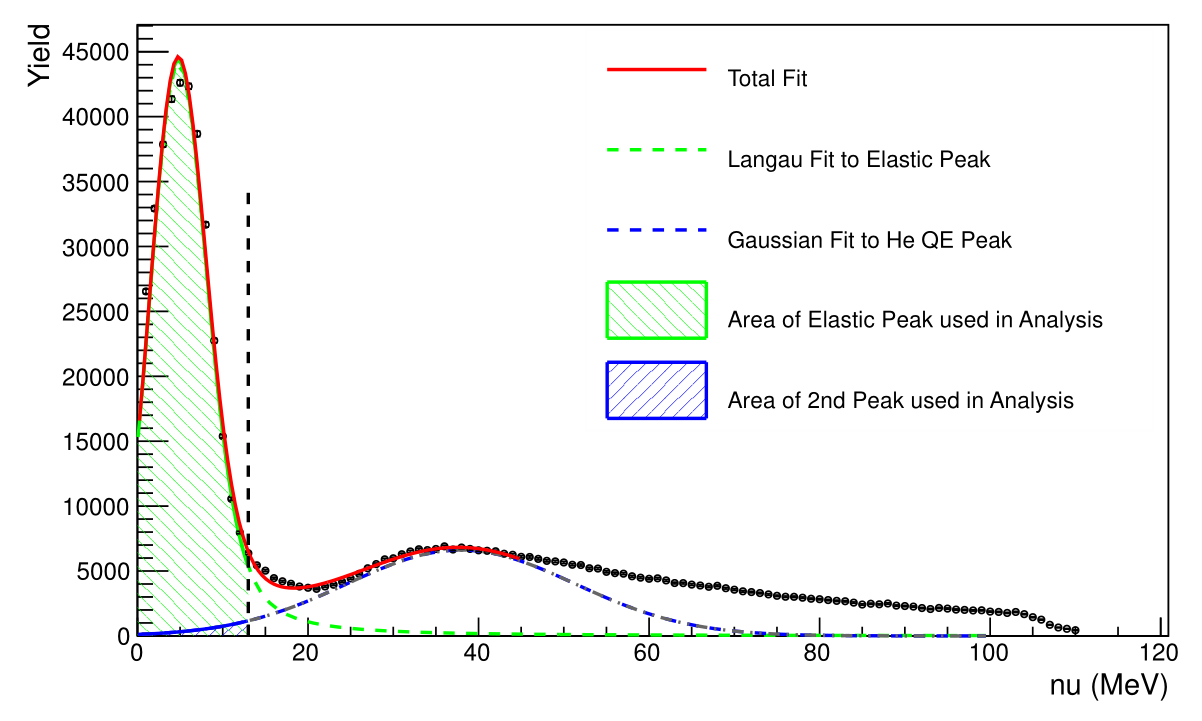
\includegraphics[width=\textwidth]{figs/packing-fraction-dummy.png}
    \caption{Fit for dummy target.}
  \end{subfigure}
  \begin{subfigure}[t]{0.46\textwidth}
    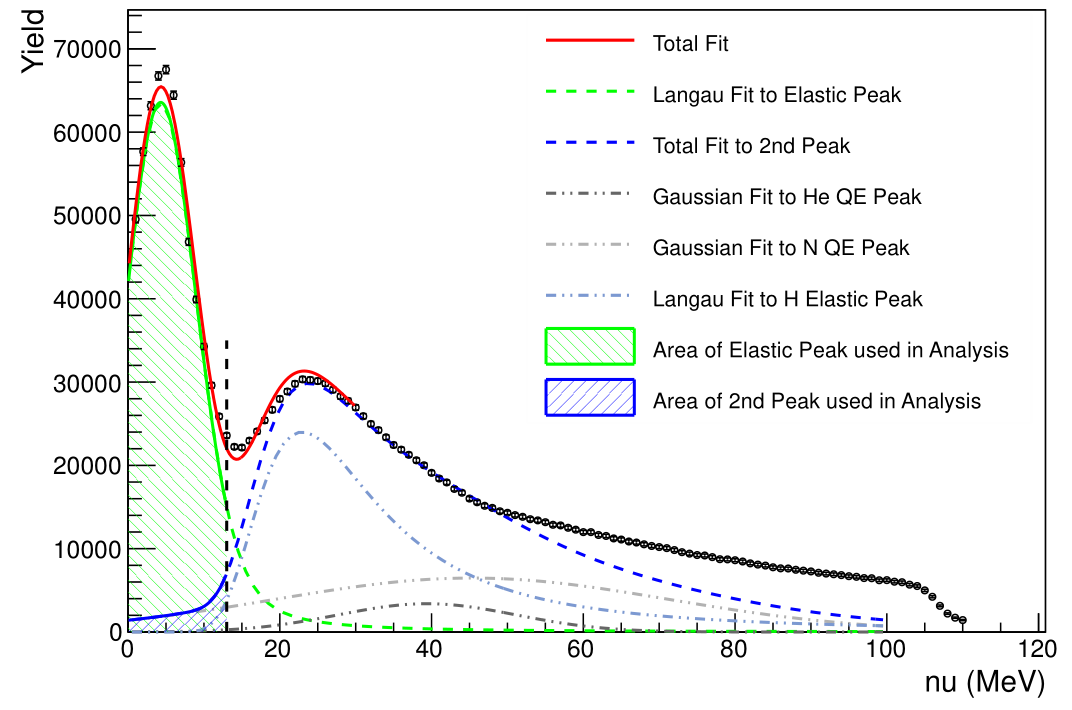
\includegraphics[width=\textwidth]{figs/packing-fraction-production.png}
    \caption{Fit for production target.}
  \end{subfigure}
  \caption[An example of the fit of the elastic and quasi-elastic peak.]{An example of the fit of the elastic and quasi-elastic peak. Plot reproduced from \cite{Cummings2015}. \label{C7S2F6}}
\end{figure}

For the dummy target, the helium elastic peak and the quasi-elastic peak are fit separately and matched with the total spectrum. However, the situation is more complicated for the production target. The spectrum contains five contributions from the nitrogen elastic peak, the helium elastic peak, the nitrogen quasi-elastic peak, the helium quasi-elastic peak and the hydrogen elastic peak. The relative contributions: each material is determined with the help of the Quasi-Free-Scattering (QFS) model \cite{Lightbody1988}.

The packing fraction analysis is discussed in Ref. \cite{Cummings2015} in detail and the results are summarized in \cref{C7S3T1} for each kinematic setting. Since the target material need to be replaced due to radiation damage, we prepared a few samples of the material. The ``Material ID'' in the table is used to distinguish these samples. The average packing fraction of the target material is $\sim$0.5 with an uncertainty of $0.01\sim0.03$.

\begin{table}[tb!]
  \centering
  \newcolumntype{C}[1]{>{\centering\arraybackslash}m{#1}}
  \begin{tabular}{|C{2.0cm}|C{2.0cm}|C{2.0cm}|C{2.0cm}|C{2.5cm}|}
    \hline
    Beam Energy & Field Strength & Field Angle & Material ID & Packing Fraction \\ \hline
    2.254 GeV & 2.5 T & \SI{90}{\degree} & 7 & 0.461$\pm$0.010 \\ \hline
    2.254 GeV & 2.5 T & \SI{90}{\degree} & 8 & 0.704$\pm$0.012 \\ \hline
    1.710 GeV & 2.5 T & \SI{90}{\degree} & 7 & 0.477$\pm$0.006 \\ \hline
    1.710 GeV & 2.5 T & \SI{90}{\degree} & 8 & 0.468$\pm$0.009 \\ \hline
    1.157 GeV & 2.5 T & \SI{90}{\degree} & 11 & 0.444$\pm$0.029 \\ \hline
    1.157 GeV & 2.5 T & \SI{90}{\degree} & 12 & 0.456$\pm$0.030 \\ \hline
    1.157 GeV & 2.5 T & \SI{90}{\degree} & 14 & 0.264$\pm$0.007 \\ \hline
    2.254 GeV & 5.0 T & \SI{0}{\degree} & 17 & 0.507$\pm$0.009 \\ \hline
    2.254 GeV & 5.0 T & \SI{0}{\degree} & 18 & 0.533$\pm$0.011 \\ \hline
    2.254 GeV & 5.0 T & \SI{90}{\degree} & 19 & 0.605$\pm$0.026 \\ \hline
    2.254 GeV & 5.0 T & \SI{90}{\degree} & 20 & 0.595$\pm$0.032 \\ \hline
  \end{tabular}
  \caption[Packing fraction results.]{Packing fraction results for each kinematic setting. Material 14 is used with a special target cell which is shorter than the normal ones. Table reproduced from \cite{Cummings2015}. \label{C7S3T1}}
\end{table}

\section{Dilution Analysis}
\label{C7S4}

The detected events from polarized electron scattering are diluted by the electrons scattered from the unpolarized material such as the nitrogen and helium nuclei in the target. Thus, the measured asymmetry need to be corrected by a factor $f$ which is referred as the dilution factor to retrieve the physics asymmetry as shown in \cref{C7S1E3}.

If the yield of the electrons scattered by unpolarized materials is denoted as $Y_{\mathrm{bg}}$, the raw asymmetry can be rewritten as:
\begin{equation} \label{C7S4E1}
A_{\mathrm{raw}} = \frac{Y^+-Y^-}{Y^++Y^-+Y_{\mathrm{bg}}}.
\end{equation}
The ammonia target used in this experiment contains ammonia beads, liquid helium and aluminum foil as caps, thus the $Y_{\mathrm{bg}}$ can be decomposed as:
\begin{equation} \label{C7S4E2}
Y_{\mathrm{bg}} = Y_{\mathrm{N}}+Y_{\mathrm{He}}+Y_{\mathrm{Al}}.
\end{equation}
Comparing \cref{C7S1E4} and \cref{C7S4E1}, the dilution factor be expressed as:
\begin{equation} \label{C7S4E3}
f = 1-\frac{Y_{\mathrm{bg}}}{Y_{\mathrm{target}}},
\end{equation}
where $Y_{\mathrm{target}}$ is given by \cref{C7S3E2}.

In \cref{C7S3E6}, we have already known that the yield of a given material is proportional to the corresponding cross-section, thus $Y_{\mathrm{bg}}$ can be rewritten as:
\begin{equation} \label{C7S4E4}
Y_{\mathrm{bg}} = AN_A\left(\frac{\rho_{\mathrm{NH_3}}L_{\mathrm{cell}}p_f}{M_{\mathrm{NH_3}}}\sigma_{\mathrm{N}}+\frac{\rho_{\mathrm{He}}(L_{\mathrm{total}}-p_fL_{\mathrm{cell}})}{M_{\mathrm{He}}}\sigma_{\mathrm{He}}+\frac{\rho_{\mathrm{Al}}L_{\mathrm{Al}}}{M_{\mathrm{Al}}}\sigma_{\mathrm{Al}}\right),
\end{equation}
where $p_f$ is the packing fraction as mentioned in \Cref{C7S3}, $A$ is the acceptance factor and $N_A$ is the Avogadro's number.

During the experiment, several different target materials were used to determine the unpolarized background contribution $Y_{\mathrm{bg}}$. These targets included a dummy cell, which can be used to estimate the aluminum contribution, and a carbon target, which can be scaled using cross-section models to approximate the nitrogen contribution. Data were also collected with the pure liquid helium in the target nose, which can be used to estimate the helium background. The yields for these runs can be written in terms of the corresponding materials:
\begin{equation} \label{C7S4E5}
Y_{\mathrm{empty}} = AN_A\left(\frac{\rho_{\mathrm{He}}L_{\mathrm{total}}}{M_{\mathrm{He}}}\sigma_{\mathrm{He}}\right),
\end{equation}
\begin{align} \label{C7S4E6}
Y_{\mathrm{dummy}} & = AN_A\left(\frac{\rho_{\mathrm{He}}L_{\mathrm{total}}}{M_{\mathrm{He}}}\sigma_{\mathrm{He}}+\frac{\rho_{\mathrm{Al}}L_{\mathrm{Al}}}{M_{\mathrm{Al}}}\sigma_{\mathrm{Al}}\right), \\ \label{C7S4E7}
Y_{\mathrm{carbon}} & = AN_A\left(\frac{\rho_{\mathrm{He}}(L_{\mathrm{total}}-L_{\mathrm{C}})}{M_{\mathrm{He}}}\sigma_{\mathrm{He}}+\frac{\rho_{\mathrm{C}}L_{\mathrm{C}}}{M_{\mathrm{C}}}\sigma_{\mathrm{C}}\right),
\end{align}
where $L_{\mathrm{C}}$ is the length of the carbon target.

The $Y_{\mathrm{Al}}$ is extracted from the dummy yield and the empty yield:
\begin{equation} \label{C7S4E8}
Y_{\mathrm{Al}} = Y_{\mathrm{dummy}}-Y_{\mathrm{empty}},
\end{equation}
and the $Y_{\mathrm{He}}$ is extracted from the empty yield:
\begin{equation} \label{C7S4E9}
Y_{\mathrm{He}} = \left(1-\frac{L_{\mathrm{cell}}}{L_{\mathrm{total}}}p_f\right)Y_{\mathrm{empty}}.
\end{equation}
The $Y_{\mathrm{N}}$ is extracted from the carbon yield by scaling the carbon yield with the cross-section ratio $\sigma_{\mathrm{N}}/\sigma_{\mathrm{C}}$. The model from Ref. \cite{Bosted2008} is used to calculate the cross-section ratio. Thus, the nitrogen contamination can be expressed as:
\begin{equation} \label{C7S4E10}
Y_{\mathrm{N}} = \frac{\sigma_{\mathrm{N}}}{\sigma_{\mathrm{C}}}p_f\frac{\rho_{\mathrm{NH_3}}L_{\mathrm{cell}}M_{\mathrm{C}}}{\rho_{\mathrm{C}}L_{\mathrm{C}}M_{\mathrm{NH_3}}}\left(Y_{\mathrm{carbon}}-\frac{L_{\mathrm{total}}-L_{\mathrm{C}}}{L_{\mathrm{total}}}Y_{\mathrm{empty}}\right).
\end{equation}
The dilution factor can be calculated via \cref{C7S4E3,C7S4E8,C7S4E9,C7S4E10}.

Since the dilution study is still on-going, a preliminary dilution factor is extracted using the cross-sections. The model from Ref. \cite{Bosted2008} is used to calculate the cross-sections for various target materials. In terms of cross-sections, the dilution factor can be expressed as:
\begin{equation} \label{C7S4E11}
f = \cfrac{3\,\cfrac{\rho_{\mathrm{NH_3}}L_{\mathrm{cell}}\,p_f}{M_{\mathrm{NH_3}}}\,\sigma_{\mathrm{H}}}{\cfrac{\rho_{\mathrm{NH_3}}L_{\mathrm{cell}}\,p_f}{M_{\mathrm{NH_3}}}(\sigma_{\mathrm{N}}+3\sigma_{\mathrm{H}})+\cfrac{\rho_{\mathrm{He}}L_{\mathrm{cell}}(1-p_f)}{M_{\mathrm{He}}}\sigma_{\mathrm{He}}+\cfrac{\rho_{\mathrm{Al}}L_{\mathrm{Al}}}{M_{\mathrm{Al}}}\sigma_{\mathrm{Al}}}.
\end{equation}

The dilution factors calculated via \cref{C7S4E11} for each kinematic setting are shown in \Cref{C7S4F1,C7S4F2,C7S4F3,C7S4F4,C7S4F5,C7S4F6}. The packing fractions used in the calculation are taken from \cref{C7S3T1}. Material 19 and 20 are also used in the $E_{\mathrm{beam}}=3.350$ GeV setting. However, no packing fraction data were collected during this setting so the packing fractions from the kinematic setting with 2.253 GeV beam energy and 5.0 T transverse target field are used in the dilution factor calculation.

\begin{figure}[h!]
  \centering
  \begin{subfigure}[t]{0.49\textwidth}
    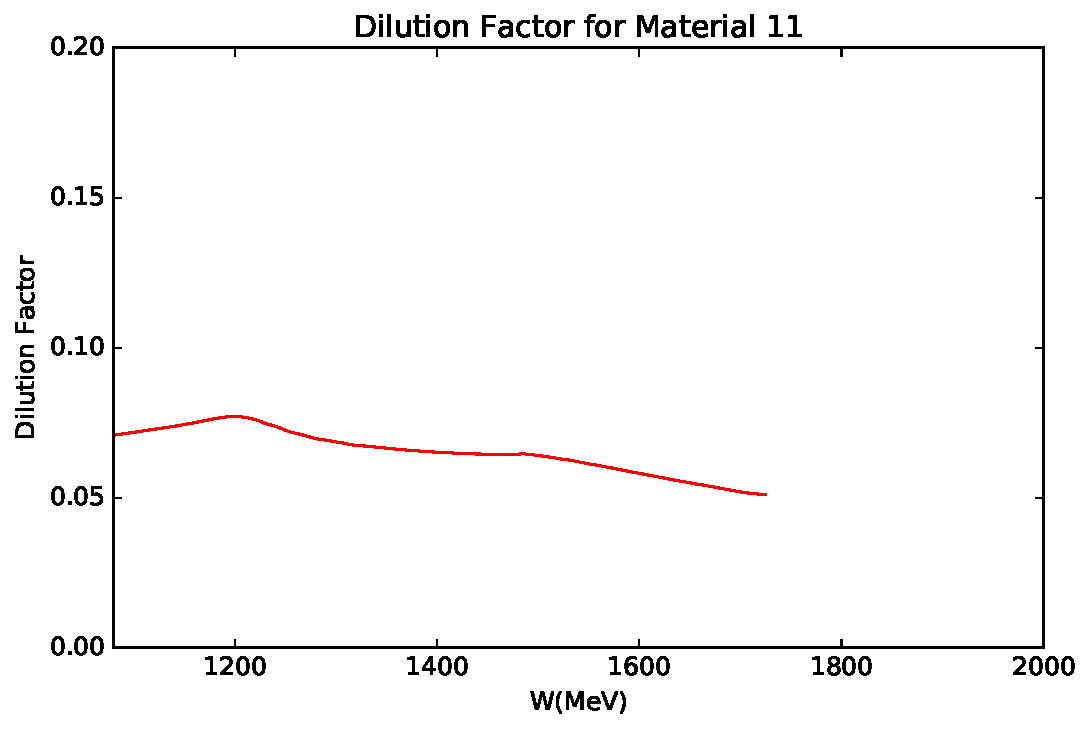
\includegraphics[width=\textwidth]{figs/dilution-11572590-11.pdf}
  \end{subfigure}
  \begin{subfigure}[t]{0.49\textwidth}
    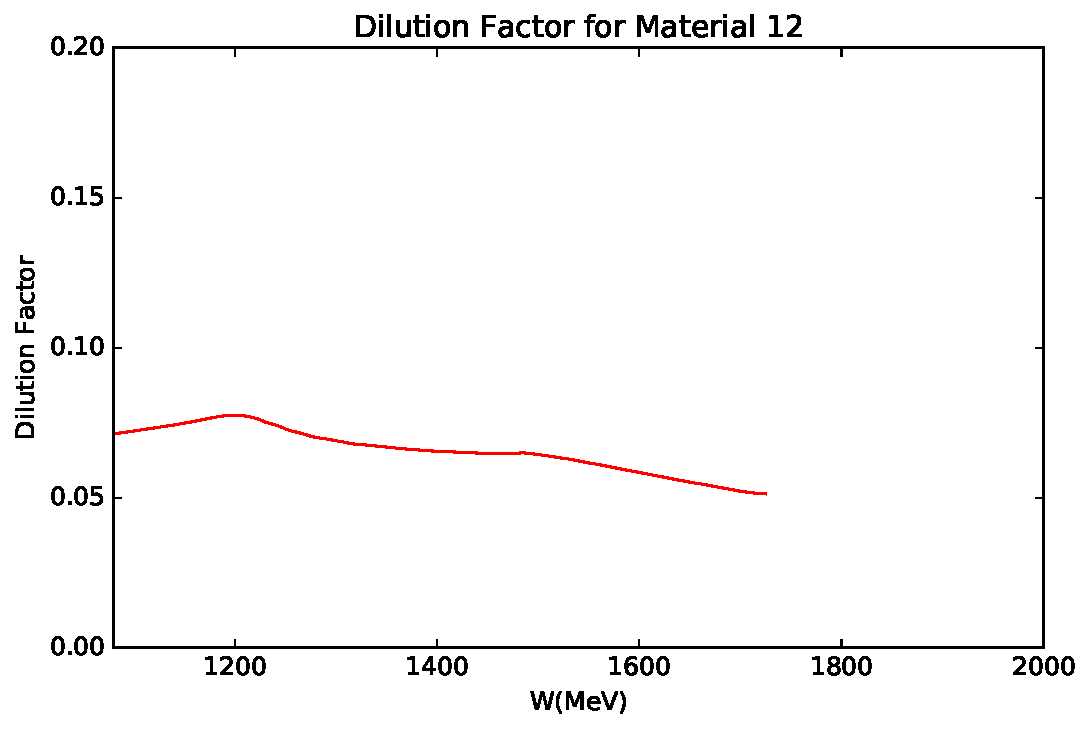
\includegraphics[width=\textwidth]{figs/dilution-11572590-12.pdf}
  \end{subfigure}
  \begin{subfigure}[t]{0.49\textwidth}
    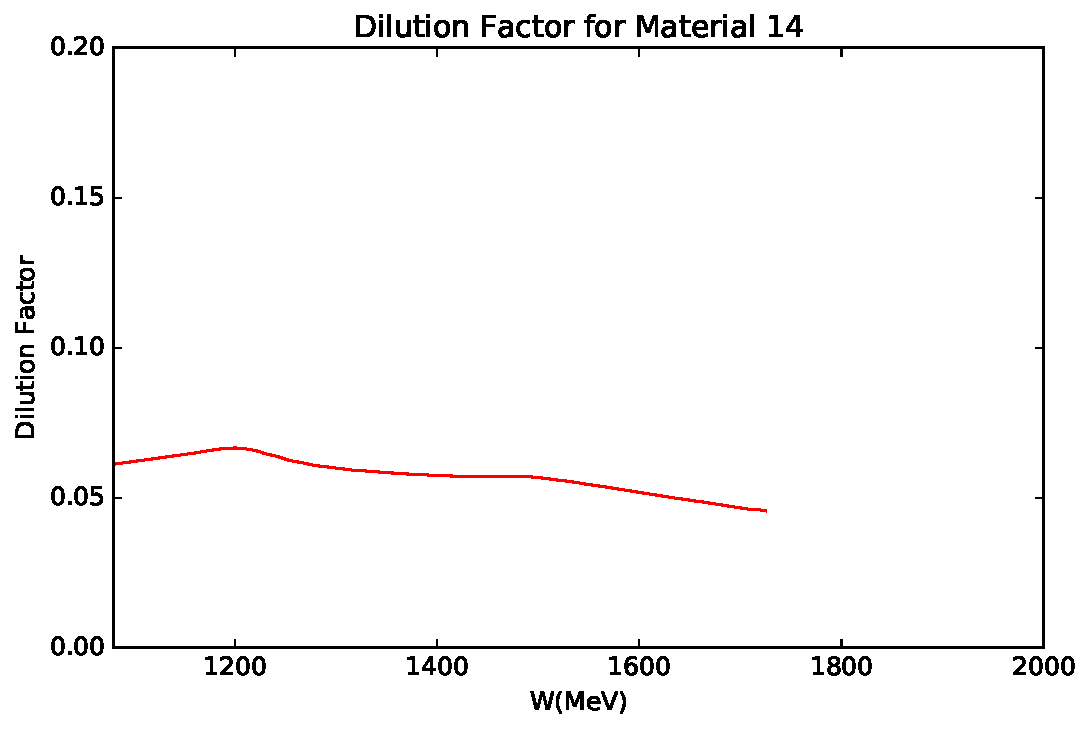
\includegraphics[width=\textwidth]{figs/dilution-11572590-14.pdf}
  \end{subfigure}
  \caption[Dilution factors with $E=1.157$ GeV and $B=2.5$ T.]{Preliminary dilution factors of the kinematic setting with 1.157 GeV beam energy and 2.5 T transverse target field. \label{C7S4F1}}
\end{figure}

\begin{figure}[h!]
  \centering
  \begin{subfigure}[t]{0.49\textwidth}
    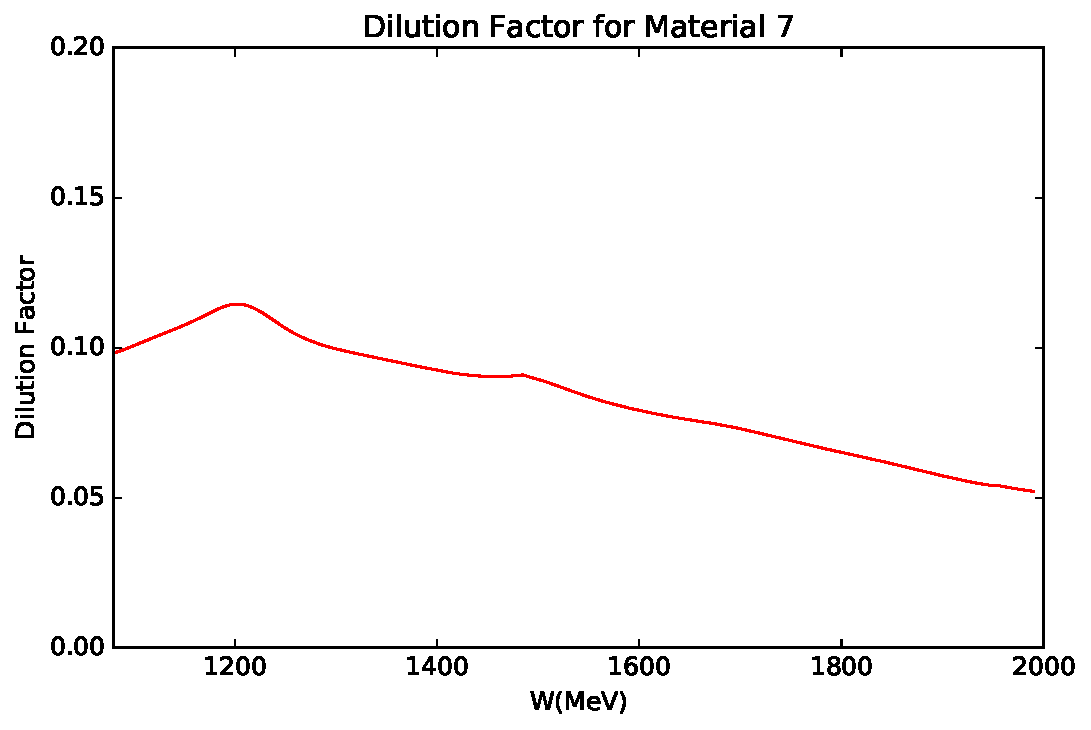
\includegraphics[width=\textwidth]{figs/dilution-17102590-7.pdf}
  \end{subfigure}
  \begin{subfigure}[t]{0.49\textwidth}
    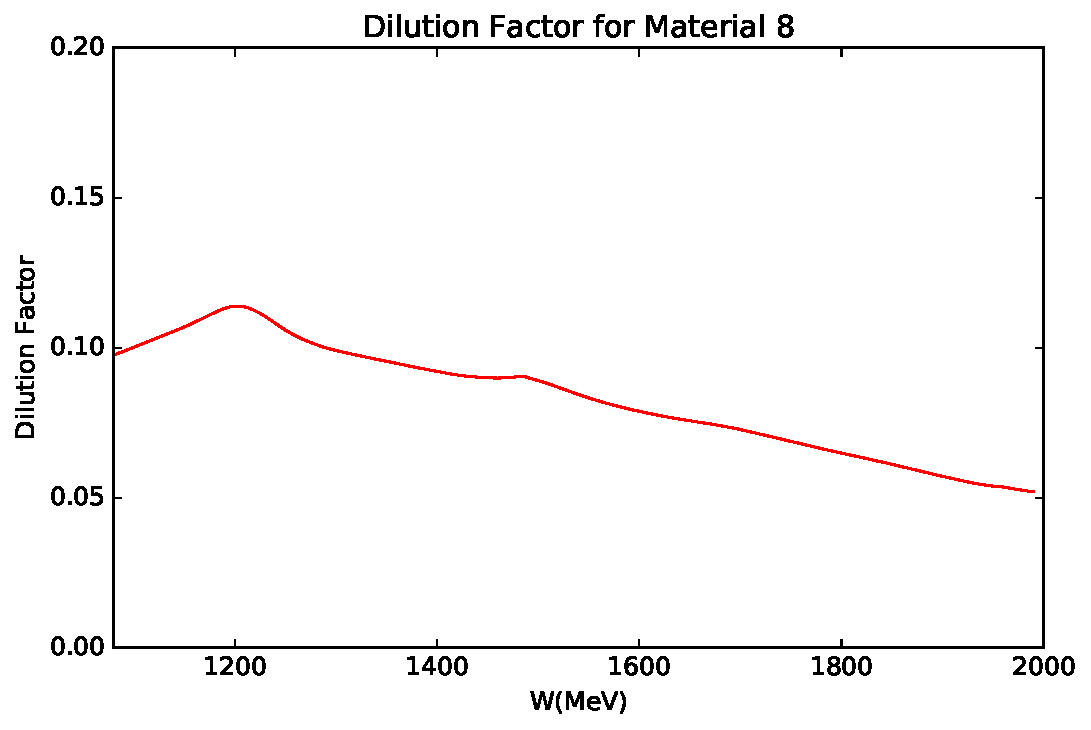
\includegraphics[width=\textwidth]{figs/dilution-17102590-8.pdf}
  \end{subfigure}
  \caption[Dilution factors with $E=1.710$ GeV and $B=2.5$ T.]{Preliminary dilution factors of the kinematic setting with 1.710 GeV beam energy and 2.5 T transverse target field. \label{C7S4F2}}
\end{figure}

\begin{figure}[p!]
  \centering
  \begin{subfigure}[t]{0.49\textwidth}
    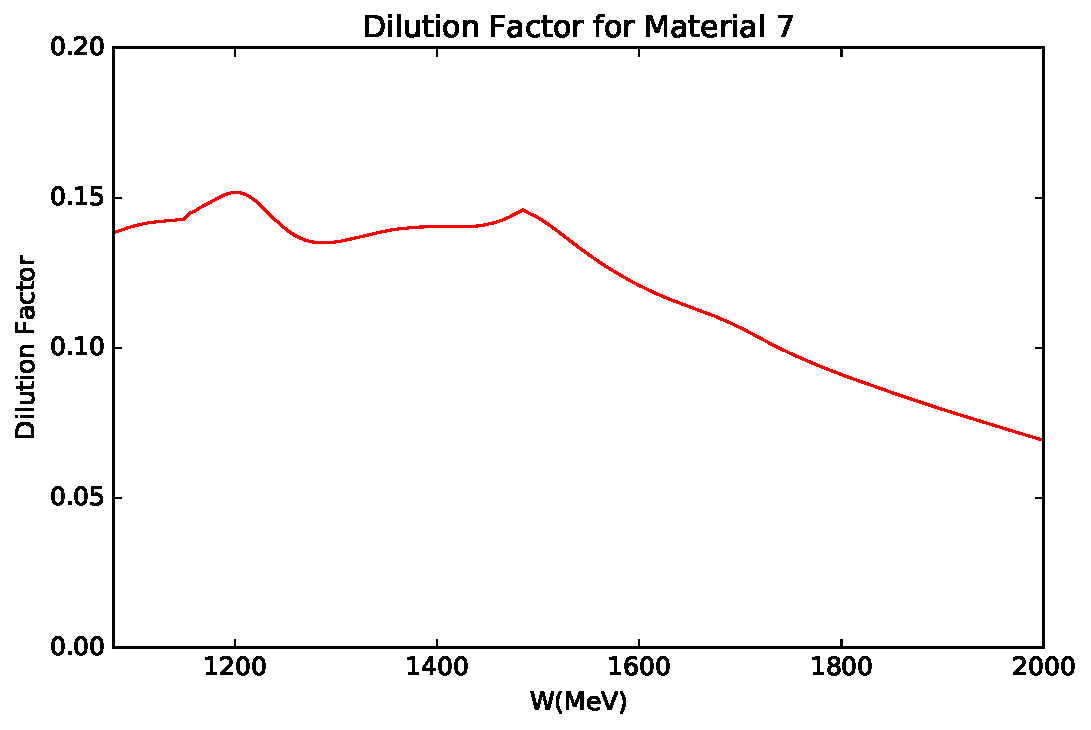
\includegraphics[width=\textwidth]{figs/dilution-22532590-7.pdf}
  \end{subfigure}
  \begin{subfigure}[t]{0.49\textwidth}
    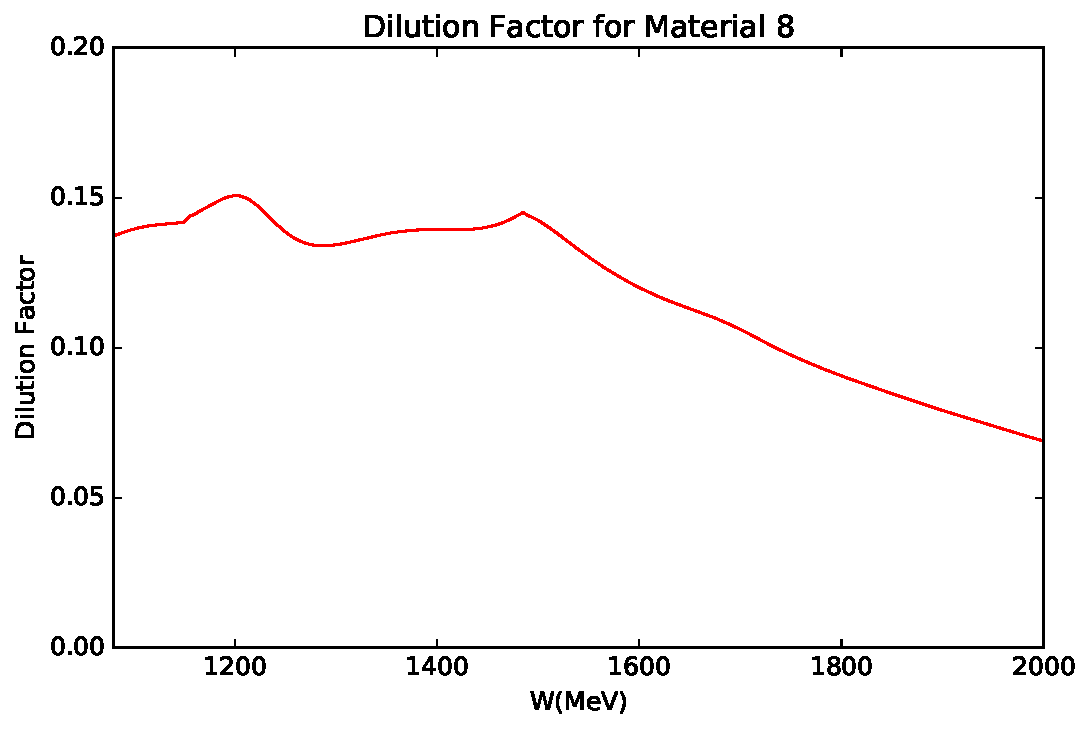
\includegraphics[width=\textwidth]{figs/dilution-22532590-8.pdf}
  \end{subfigure}
  \caption[Dilution factors with $E=2.253$ GeV and $B=2.5$ T.]{Preliminary dilution factors of the kinematic setting with 2.253 GeV beam energy and 2.5 T transverse target field. \label{C7S4F3}}
\end{figure}

\begin{figure}[p!]
  \centering
  \begin{subfigure}[t]{0.49\textwidth}
    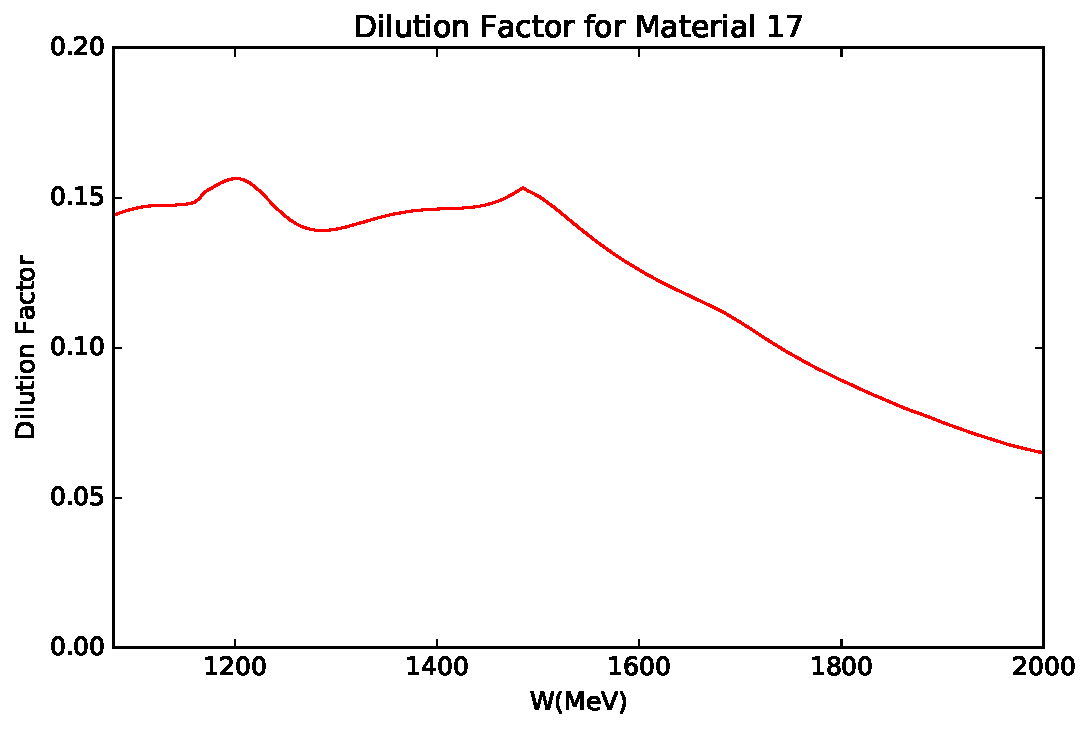
\includegraphics[width=\textwidth]{figs/dilution-22535000-17.pdf}
  \end{subfigure}
  \begin{subfigure}[t]{0.49\textwidth}
    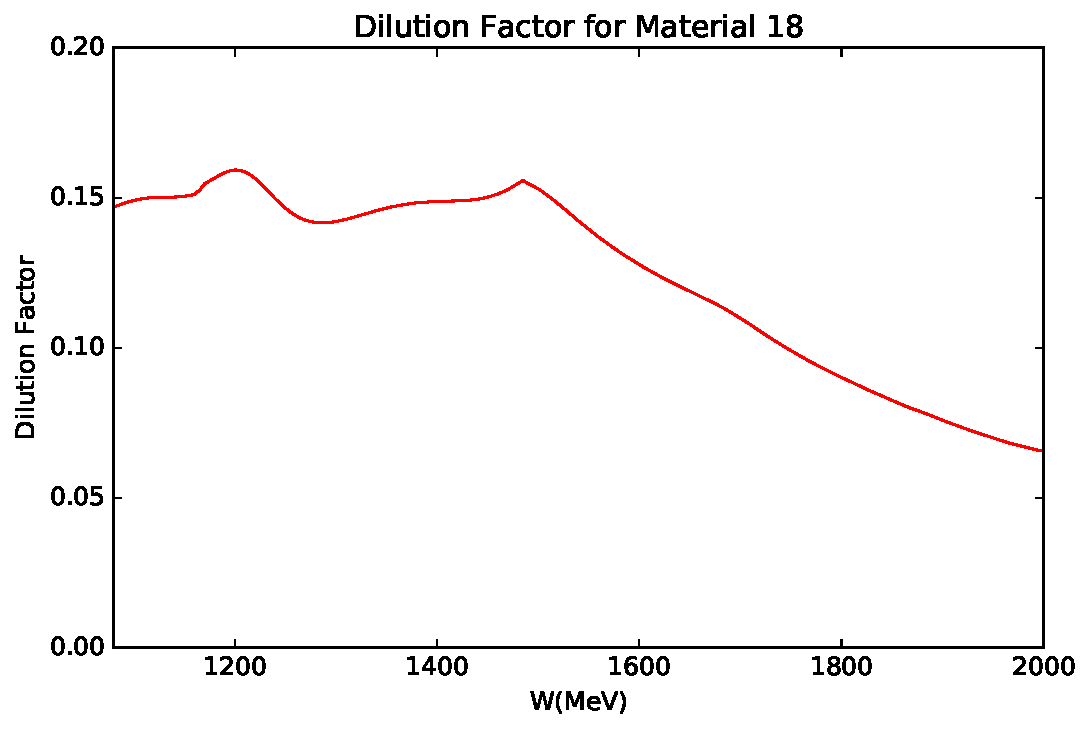
\includegraphics[width=\textwidth]{figs/dilution-22535000-18.pdf}
  \end{subfigure}
  \caption[Dilution factors with $E=2.253$ GeV and $B=5.0$ T (longitudinal).]{Preliminary dilution factors of the kinematic setting with 2.253 GeV beam energy and 5.0 T longitudinal target field. \label{C7S4F4}}
\end{figure}

\begin{figure}[p!]
  \centering
  \begin{subfigure}[t]{0.49\textwidth}
    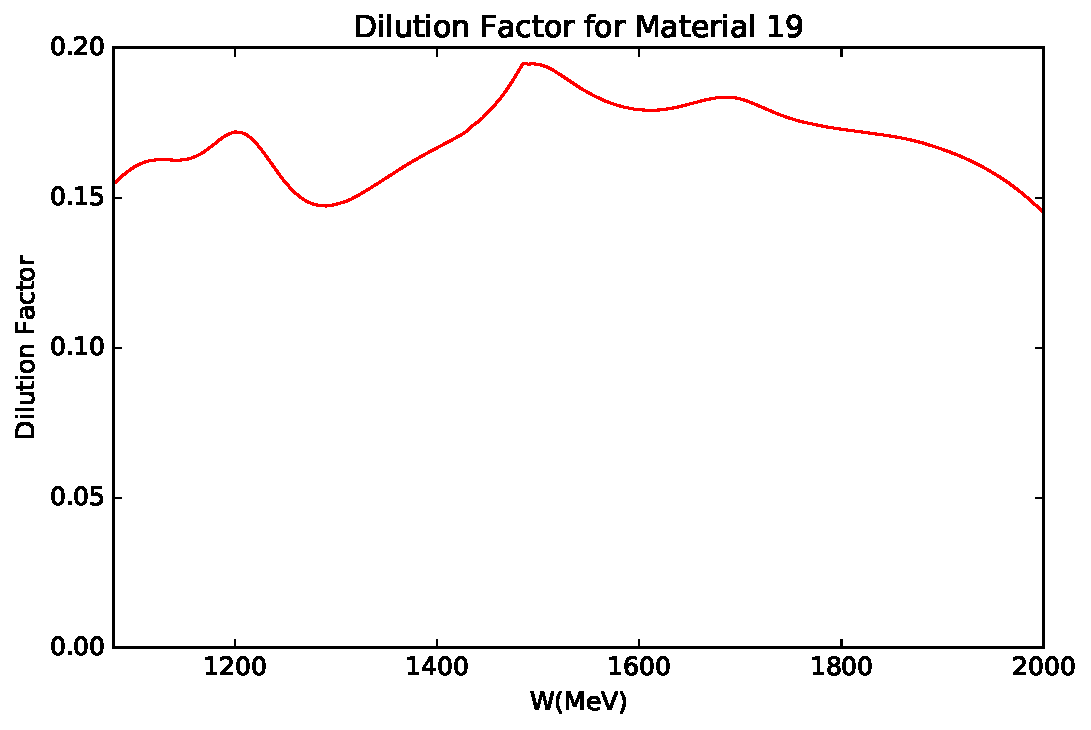
\includegraphics[width=\textwidth]{figs/dilution-22535090-19.pdf}
  \end{subfigure}
  \begin{subfigure}[t]{0.49\textwidth}
    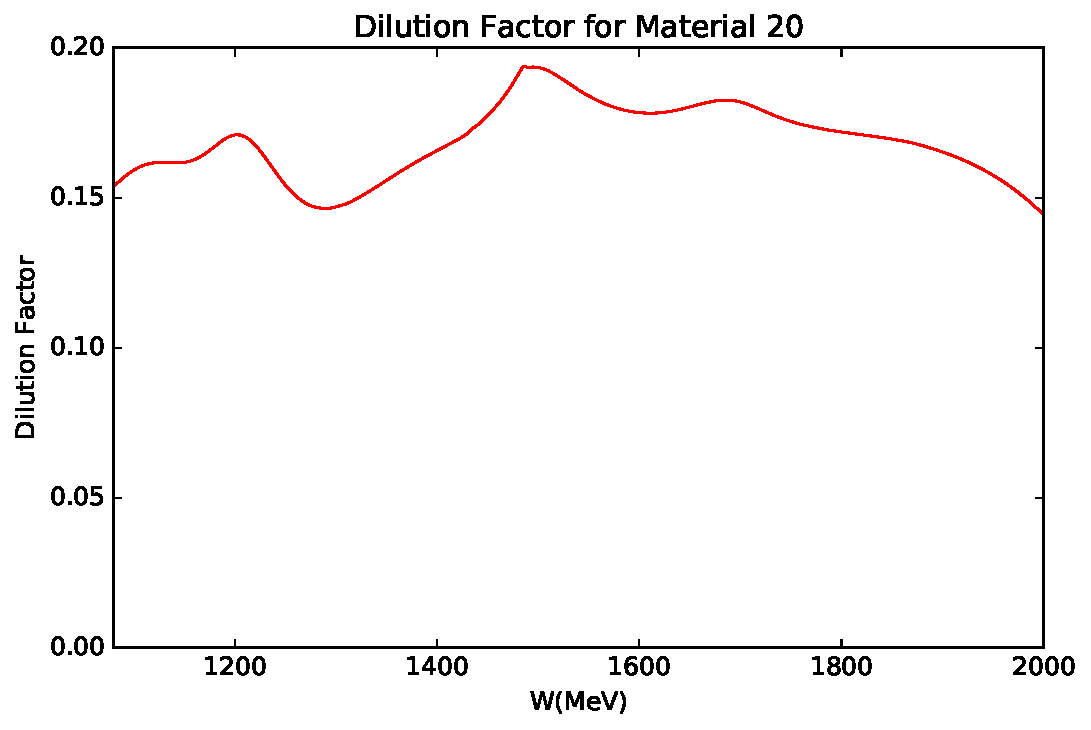
\includegraphics[width=\textwidth]{figs/dilution-22535090-20.pdf}
  \end{subfigure}
  \caption[Dilution factors with $E=2.253$ GeV and $B=5.0$ T (transverse).]{Preliminary dilution factors of the kinematic setting with 2.253 GeV beam energy and 5.0 T transverse target field. \label{C7S4F5}}
\end{figure}

\begin{figure}[h!]
  \centering
  \begin{subfigure}[t]{0.49\textwidth}
    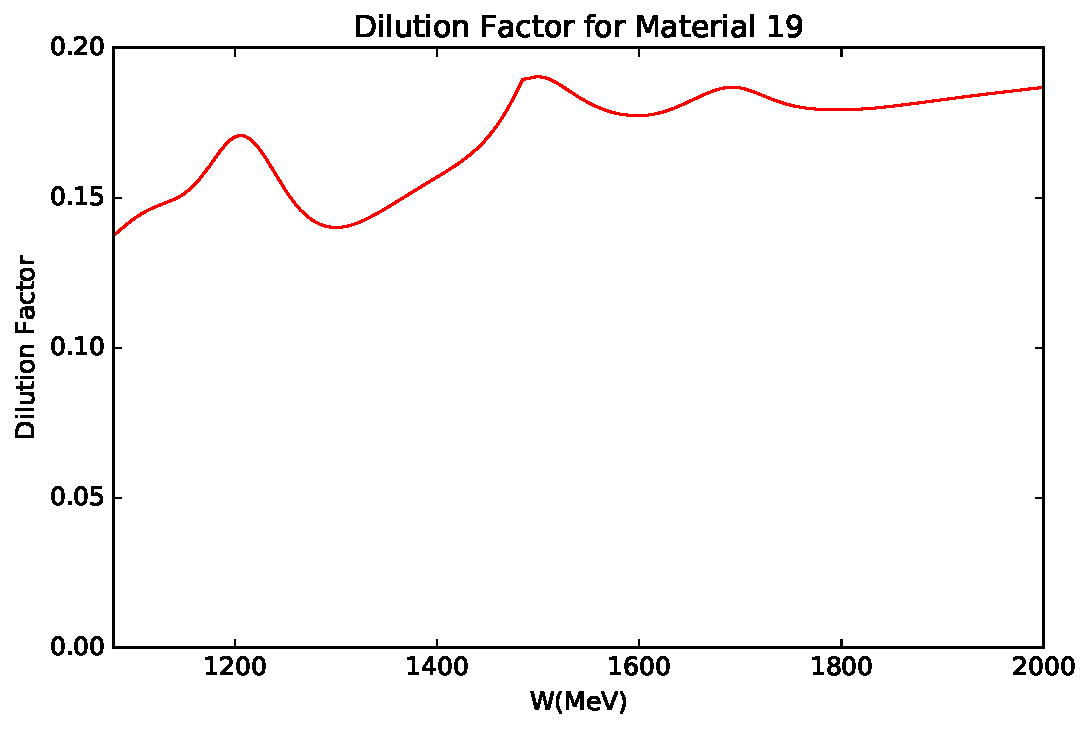
\includegraphics[width=\textwidth]{figs/dilution-33505090-19.pdf}
  \end{subfigure}
  \begin{subfigure}[t]{0.49\textwidth}
    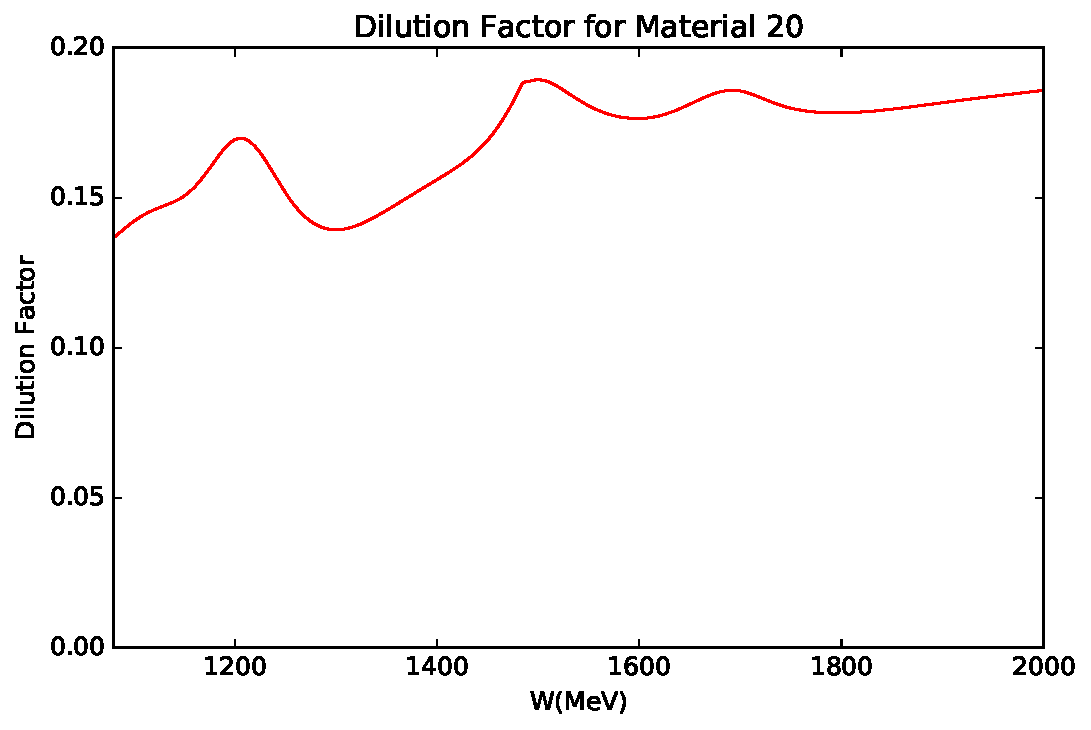
\includegraphics[width=\textwidth]{figs/dilution-33505090-20.pdf}
  \end{subfigure}
  \caption[Dilution factors with $E=3.350$ GeV and $B=2.5$ T.]{Preliminary dilution factors of the kinematic setting with 3.350 GeV beam energy and 5.0 T transverse target field. \label{C7S4F6}}
\end{figure}

%%%%%%%%%%%%%%%%%%%%%%%%%%%%%%%%%%%%%%%%%%%%%%%%%%%%%%%%%%%%%%%%%%%%%%
% -*-latex-*-
